\documentclass[10pt,twocolumn,letterpaper]{article}

\usepackage{cvpr}
\usepackage{times}
\usepackage{epsfig}
\usepackage{graphicx}
\usepackage{amsmath}
\usepackage{amssymb}
\usepackage{caption}
\usepackage{subcaption}
% Include other packages here, before hyperref.

% If you comment hyperref and then uncomment it, you should delete
% egpaper.aux before re-running latex.  (Or just hit 'q' on the first latex
% run, let it finish, and you should be clear).
\usepackage[breaklinks=true,bookmarks=false]{hyperref}

\cvprfinalcopy % *** Uncomment this line for the final submission

\def\cvprPaperID{****} % *** Enter the CVPR Paper ID here
\def\httilde{\mbox{\tt\raisebox{-.5ex}{\symbol{126}}}}

% Pages are numbered in submission mode, and unnumbered in camera-ready
%\ifcvprfinal\pagestyle{empty}\fi
\pagenumbering{gobble}
\begin{document}

%%%%%%%%% TITLE
\title{Image Quilting for Texture Synthesis and Transfer}

\author{Aman Kansal\\
170050027\\
\and
Ansh Khurana\\
170050035\\
\and
Kushagra Juneja\\
170050041
}

\maketitle
%\thispagestyle{empty}

% %%%%%%%%% ABSTRACT
% \begin{abstract}
   
% \end{abstract}

%%%%%%%%% BODY TEXT
\section{Introduction}
refer abstract-intro from paper. Here we solve the problem of synthesizing a large image following the given input texture. Also, transferring the texture to another image.  
\begin{figure}[h]
\begin{center}
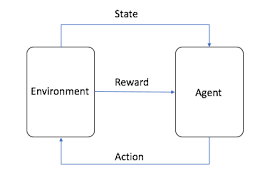
\includegraphics[scale=0.50]{resources/rl_general.png}
\end{center}
\vspace{-0.2em}
\caption{Reinforcement Learning Paradigm}
\label{fig:basic}
\end{figure}
%-------------------------------------------------------------------------
\vspace{-6pt}
\section{Method}

\subsection{Quilting}
Explain algo. Maybe add pseudocode in an algorithm block. Add figure with minimum boundary cut to explain the algo.
\begin{figure}[h]
\begin{center}
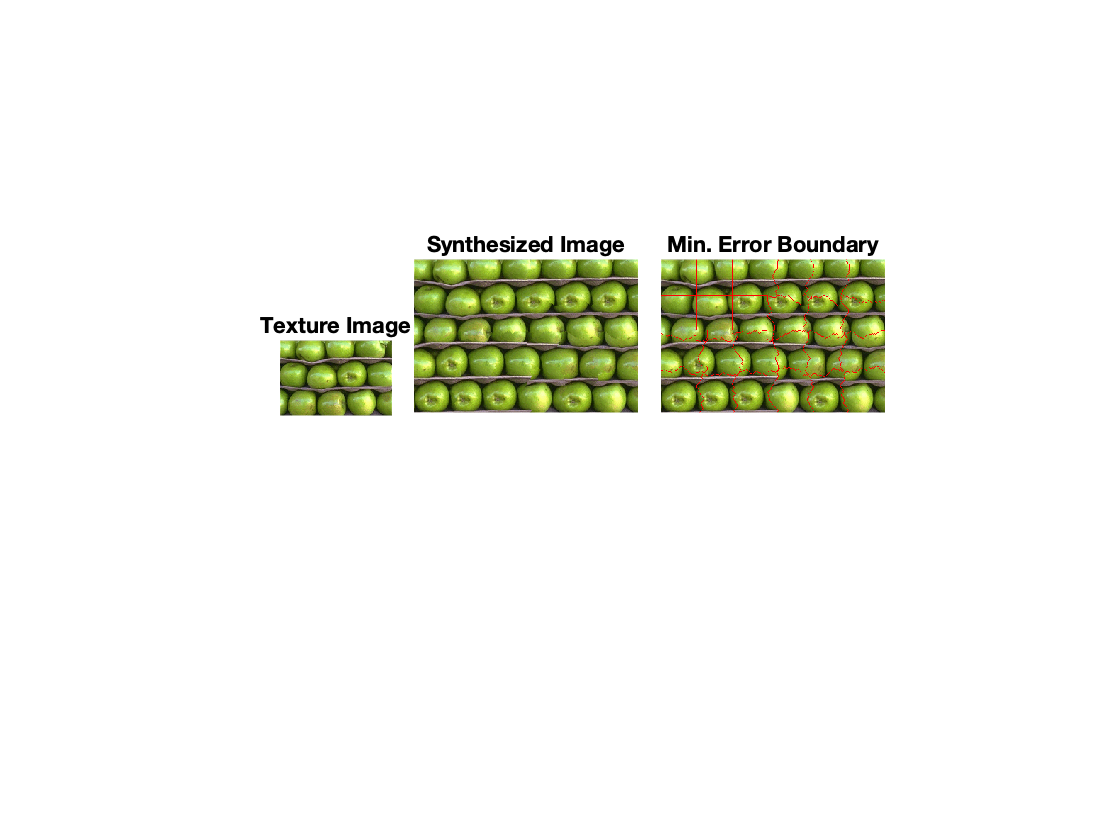
\includegraphics[trim={9cm 15cm 2cm 8cm},clip, scale=0.38]{resources/apple_boundary_example.png}
\end{center}
\vspace{-0.2em}
\caption{Boundary Cuts in Synthesis of Apple image}
\label{fig:bcut_example}
\end{figure}
% \begin{align*}
%     Q_{n}(s, a) = \left(1-\alpha_{n}\right) Q_{n-1}(s, a)+\alpha_{n}\left[r_{n}+\gamma V_{n-1}\left(y_{n}\right)\right]
% \end{align*}
%-------------------------------------------------------------------------
\subsection{Texture Transfer}
In the task of texture transfer, the input is taken in form
of small piece of texture and a target image. The aim is to
reconstruct the target image from small patches of the given
texture so that the high level information in the image is
preserved while giving it a textured appearance similar to
the input texture.

\subsubsection{Algorithm}
The algorithm for this task is similar to the quilting algo-
rithm, except that the final image is constructed in multiple
iterations, each producing a better output image than the
previous one. The output image is of the same dimensions
as the input target image. Thus, each patch in the output im-
age corresponds to a patch in the target image. After placing
the first patch (at the top-left corner say) in the output im-
age, we progressively place the next patch, stochastically
minimizing the summation of following two losses -

\begin{itemize}
    \item SSE (sum of squared errors) between the pixels in the
    new patch and those in the surrounding patches, in the
    overlap region. Call it SSE1
    \item SSE between the pixels in the new patch and the pixels
    in the corresponding patch of the target image. Call it
    SSE2
\end{itemize}
\newline
Mathematically the minimized loss is -
\begin{align}
L = \alpha *SSE1 + (1 - \alpha) *SSE2\notag
\end{align}
The paramter α, in i th iteration is heuristically kept
as $\alpha_i = 0.8*\frac{i-1}{N-1}+0.1$
where $N$ is the total number
of iterations and is ideally kept between 3 to 5. The size
of the patch is also reduced in each successive iteration
in a geometric fashion, i.e., $B_{i+1} = B_i *d$ where $d$ is
the decay rate for patch size and a hyperparameter for
the algorithm. In the successive iteration we replace the
target image by the image obtained in the previous iteration.
\newline
\newline
\textbf{Intuition behind iterative algorithm} We can observe
that in the successive iterations, in addition to reducing
the patch size, we alter the relative weights for the two
SSE’s adding more weight to maintaining continuity
accross edges. The explanation behind it is as follows -
We choose larger patches first (although still small enough
to be able to replicate target image), so as to preserve the
important components in the texture. This might reflect
some discountinuities at the edges of the block. In the
subsequent iterations, when smaller patches are being
chosen then the patches inside the previously larger patch
would tend to remain same (as they match the target imageperfectly and are inherently continuous), but the patches at
the boundary would be chosen so as the remain closer to
the previously chosen patch, while enhancing continuity
accross the boundary.

\subsection{Neural Network Style Transfer}
% Insert picture of the model
Not doing this anymore.
Deep Learning does away with the need to handcraft features for the states. In the Deep Q-Learning based approach, the state is captured by an image of the current situation of the game. %We create an image representing the current state of the game every four frames which are blended together and preprocessed.
Deep Q-Learning is an extension of function approximation for Q-Learning. Deep Q-Learning uses a deep neural network to approximate the Q values for every action, given the current state. Thus, the output layer of the Deep Q-Network has dimensions = $|A|$ (The number of actions). The best action after learning the network can be taken by calculating an argmax over the output layer. 

\begin{figure}[h]
\begin{center}
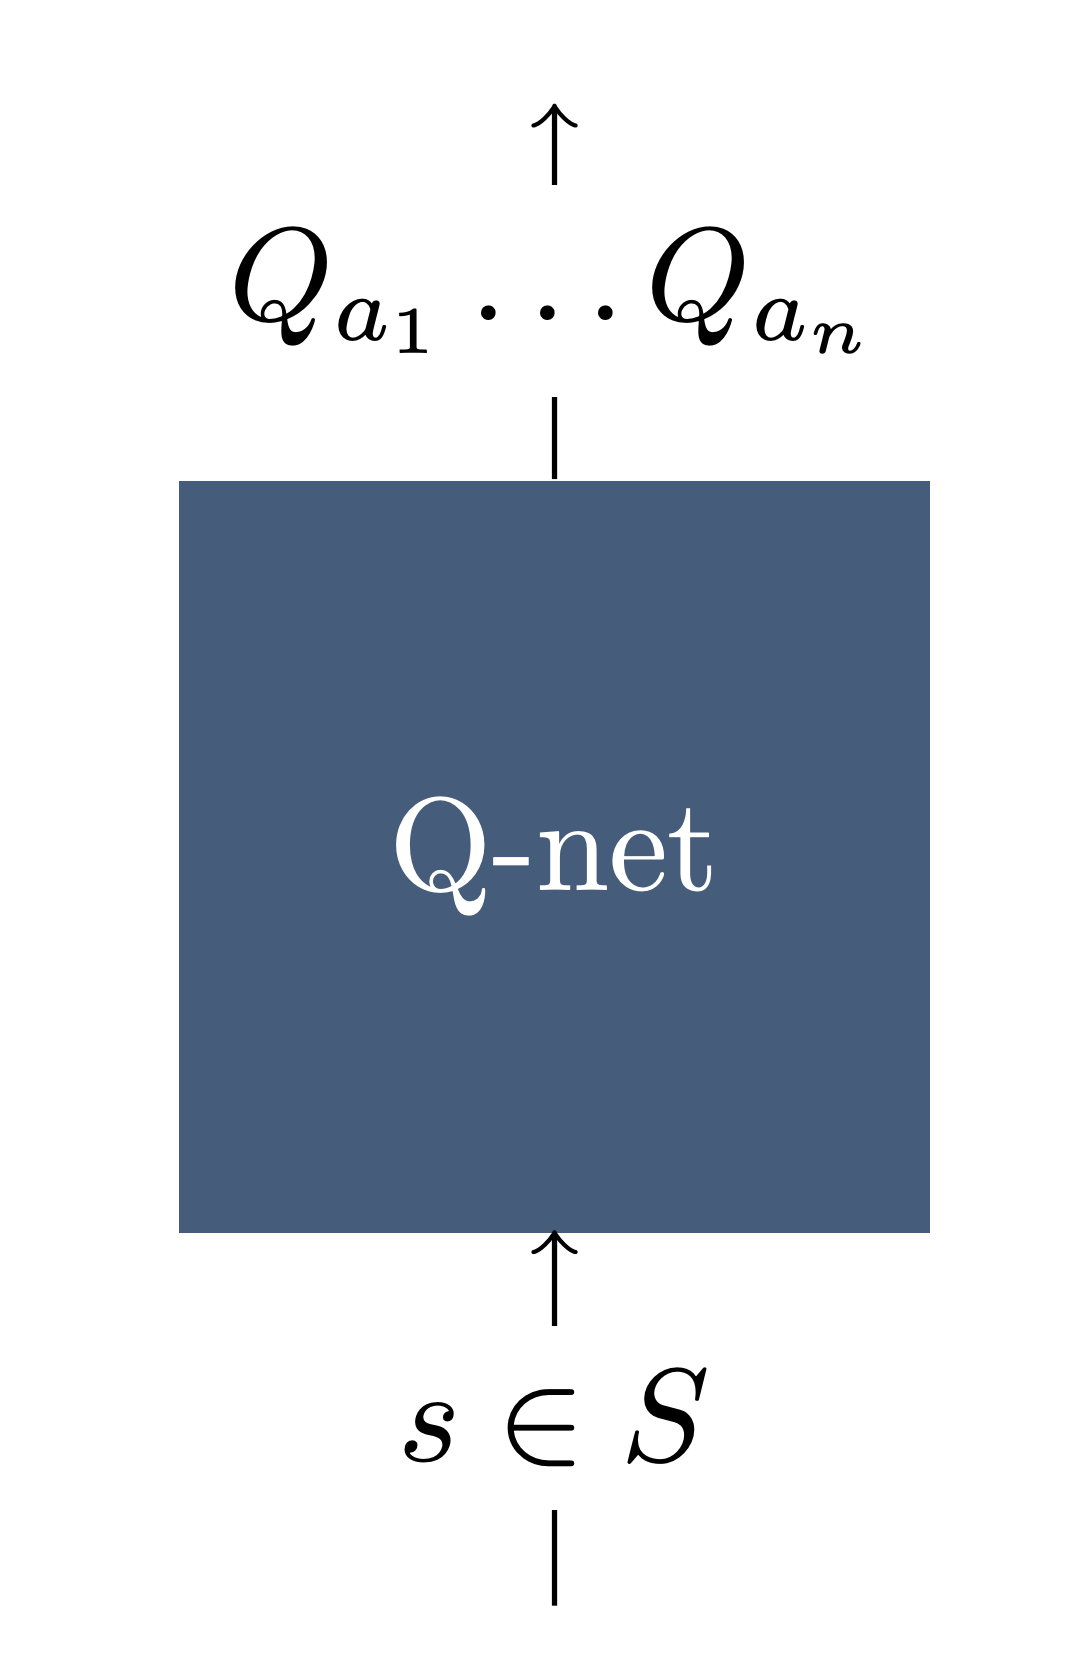
\includegraphics[scale=0.15]{resources/generalQnetwork.png}
\end{center}
\vspace{-0.2em}
\caption{A generic Deep Q-Network}
\label{fig:genericDQN}
\end{figure}
%-------------------------------------------------------------------------

\section{Experiments}
% Add parameters chosen and values of different things learning rate
\subsection{Quilting}
The effect of block size can be seen in figures x, y and z. These are our observations and here is why.
\begin{figure*}[h]
    \centering
    \begin{subfigure}[h]{0.2\textwidth}
        \centering
        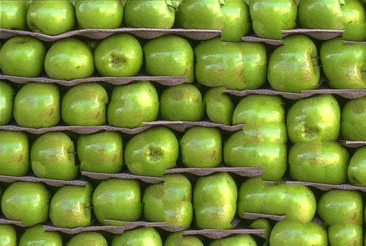
\includegraphics[scale=0.25]{../results/syn/out_apples_B_20.png}
        \caption{B=20}
    \end{subfigure}
    \hfill
    \begin{subfigure}[h]{0.2\textwidth}
       \centering
       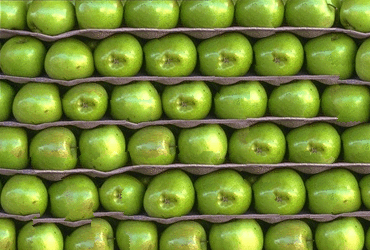
\includegraphics[scale=0.25]{../results/syn/out_apples_B_30.png}
       \caption{B=30}
   \end{subfigure}
   \hfill
   \begin{subfigure}[h]{0.2\textwidth}
       \centering
       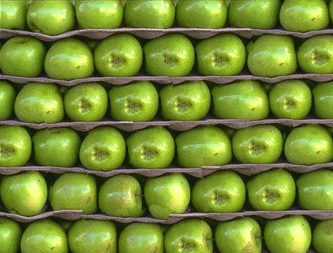
\includegraphics[scale=0.25]{../results/syn/out_apples_B_40.png}
       \caption{B=40}
   \end{subfigure}
   \begin{subfigure}[h]{0.2\textwidth}
       \centering
       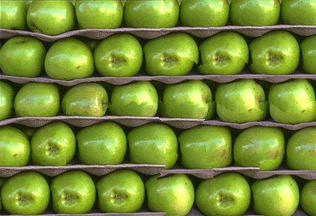
\includegraphics[scale=0.25]{../results/syn/out_apples_B_50.png}
       \caption{B=50}
   \end{subfigure}
   \caption{Effect of block size on Apples}
   \label{fig:ap_bs}
\end{figure*}

\begin{figure*}[h]
    \centering
    \begin{subfigure}[h]{0.2\textwidth}
        \centering
        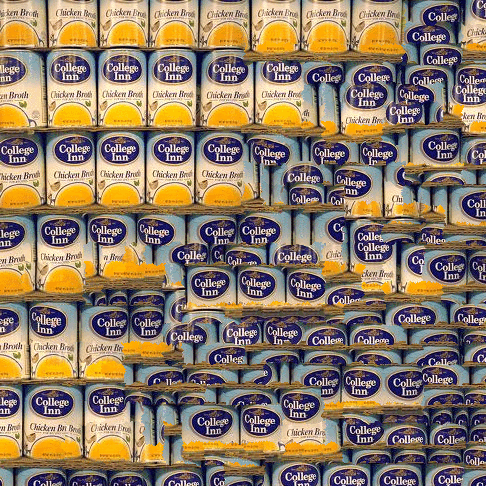
\includegraphics[scale=0.15]{../results/syn/out_cans_B_20.png}
        \caption{B=20}
    \end{subfigure}
    \hfill
    \begin{subfigure}[h]{0.2\textwidth}
       \centering
       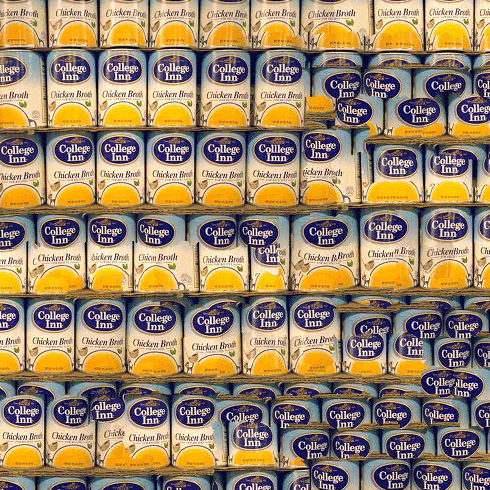
\includegraphics[scale=0.15]{../results/syn/out_cans_B_30.png}
       \caption{B=30}
   \end{subfigure}
   \hfill
   \begin{subfigure}[h]{0.2\textwidth}
       \centering
       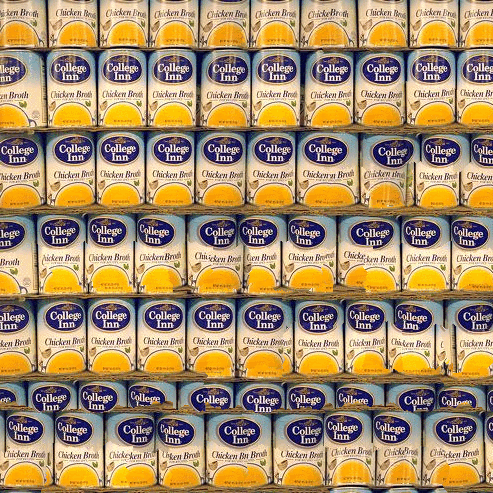
\includegraphics[scale=0.15]{../results/syn/out_cans_B_40.png}
       \caption{B=40}
   \end{subfigure}
   \begin{subfigure}[h]{0.2\textwidth}
       \centering
       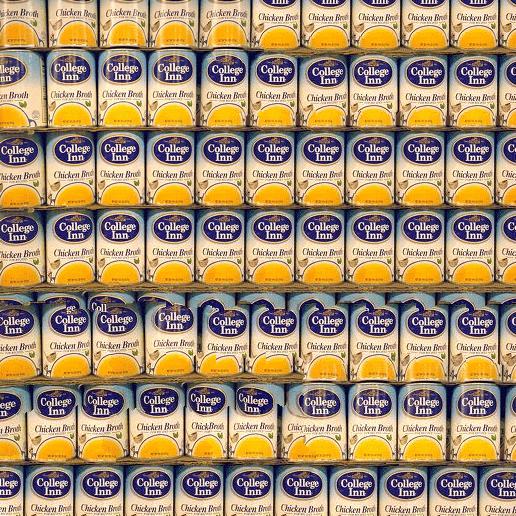
\includegraphics[scale=0.15]{../results/syn/out_cans_B_50.png}
       \caption{B=50}
   \end{subfigure}
   \caption{Effect of block size on Cans}
   \label{fig:cans_bs}
\end{figure*}

\begin{figure*}[h]
    \centering
    \begin{subfigure}[h]{0.2\textwidth}
        \centering
        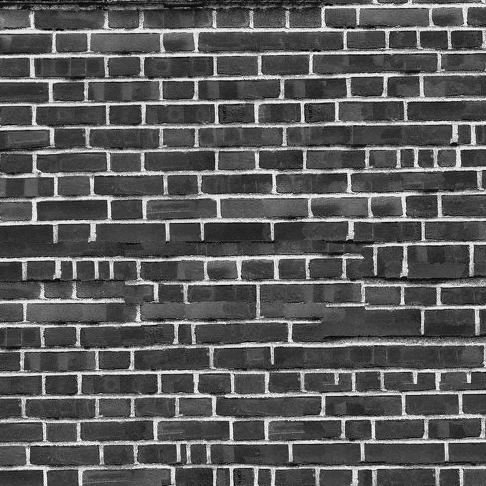
\includegraphics[scale=0.15]{../results/syn/out_brick_bw_B_20.png}
        \caption{B=20}
    \end{subfigure}
    \hfill
    \begin{subfigure}[h]{0.2\textwidth}
       \centering
       
\includegraphics[scale=0.15]{../results/syn/out_brick_bw_B_30.png}
       \caption{B=30}
   \end{subfigure}
   \hfill
   \begin{subfigure}[h]{0.2\textwidth}
       \centering
       
\includegraphics[scale=0.15]{../results/syn/out_brick_bw_B_40.png}
       \caption{B=40}
   \end{subfigure}
   \begin{subfigure}[h]{0.2\textwidth}
       \centering
       
\includegraphics[scale=0.15]{../results/syn/out_brick_bw_B_50.png}
       \caption{B=50}
   \end{subfigure}
   \caption{Effect of block size on Bricks}
   \label{fig:cans_bs}
\end{figure*}

% \begin{table}[!th]
% \begin{center}
% \begin{tabular}{|l|c|}
% \hline
% Situation & Reward \\
% \hline\hline
% Win (finish food) & +500 \\
% Lose (eaten by ghost) & -500 \\
% Eat food & +10\\
% Consume ghost & +200\\
% Idle/no food & -1\\
% \hline
% \end{tabular}
% \end{center}
% \caption{Game parameters for Q-Learning}
% \end{table}
% The features chosen for training the Approximate Q-Learning Network are: bias, number\_of\_ghosts\_1\_step\_away, distance\_to\_closest\_food
% \begin{table}[!th]
% \begin{center}
% \begin{tabular}{|l|c|c|c|c|}
% \hline
% Approach & Grid size & Avg Score & \#Epochs & Time (train)\\
% \hline\hline
% AQL & mediumClassic & 1202.7 & 50 & 5m 45s\\
% AQL & mediumGrid & 526.4 & 50 & 32s \\
% QL & smallGrid & 499.5 & 2000 & 1m 24s\\
% \hline
% \end{tabular}
% \end{center}
% \caption{Some simulations}
% \label{tab:qlres}
% \end{table}


% \begin{figure}[h]
% \begin{center}
% 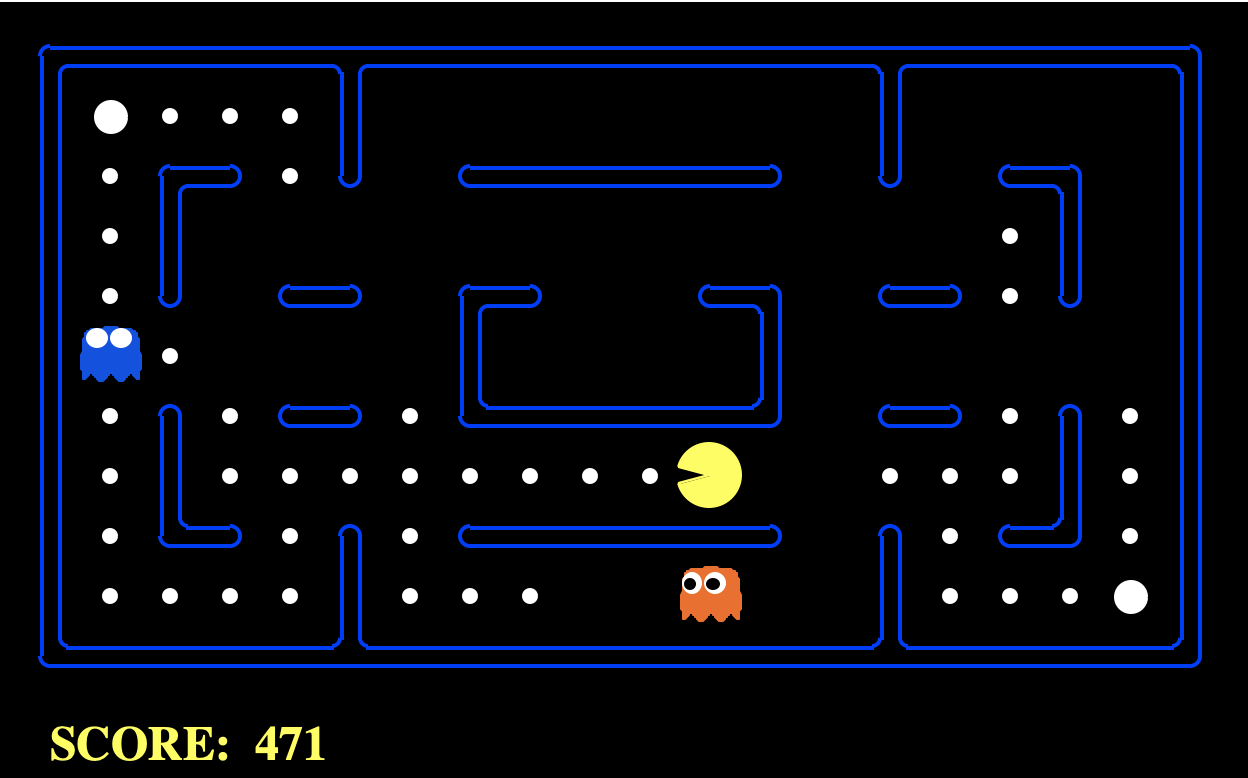
\includegraphics[scale=0.25]{resources/game_preview.png}
% \end{center}
% \vspace{-0.2em}
% \caption{Pac-Man during Training}
% \label{fig:basic}
% \end{figure}

\subsection{Transfer}
Here are the observed effects of increasing block size. Trade-off between content preservation and similarity of texture.
\begin{figure*}[h]
    \begin{center}
    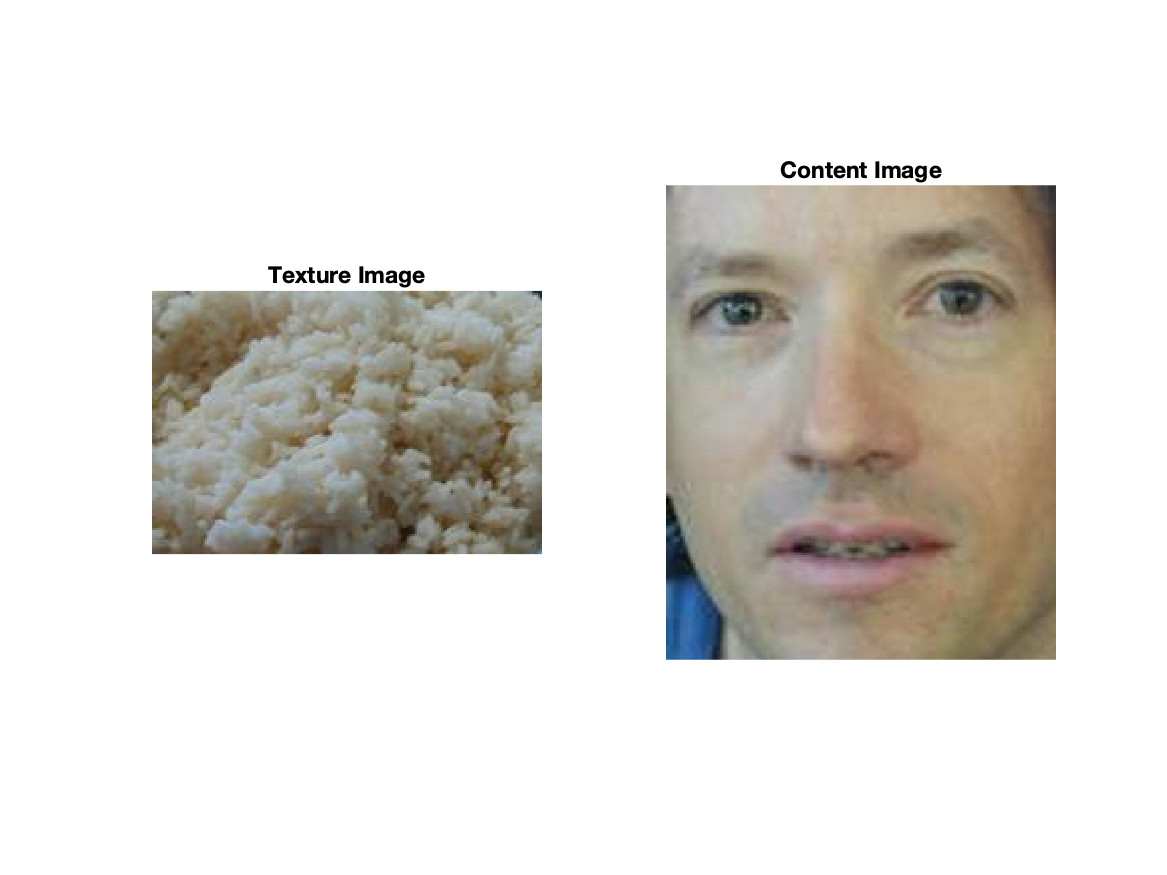
\includegraphics[trim={2cm 4cm 2cm 2cm}, clip, scale=0.5]{../results/bsize/inp_rice_bill.png}
    \end{center}
    \vspace{-0.2em}
    \caption{Rice-Bill}
    \label{fig:rice_bill}
\end{figure*}

% Block Size
\begin{figure*}[h]
    \begin{center}
    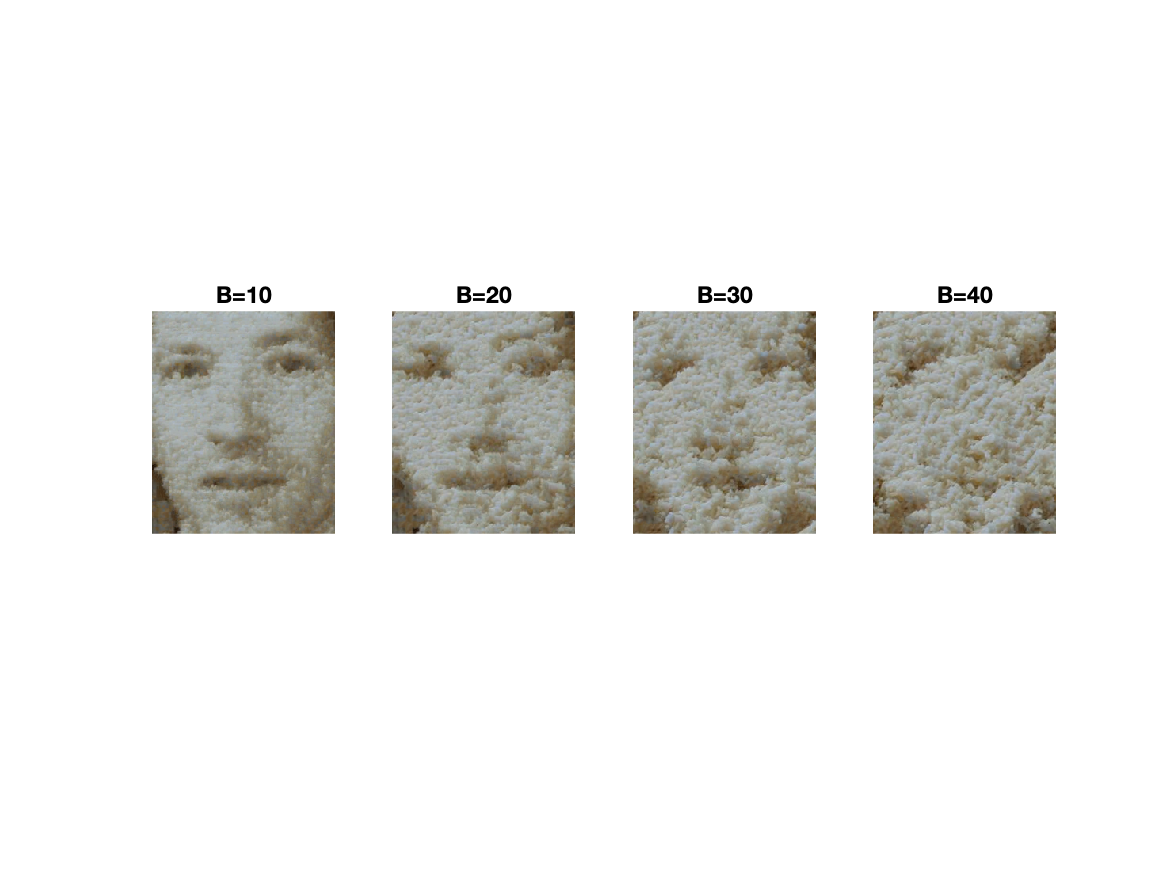
\includegraphics[trim={2cm 6cm 2cm 4cm}, clip, scale=0.9]{../results/bsize/res_rice_bill_bdr_0_800000_iter_5.png}
    \end{center}
    \vspace{-0.2em}
    \caption{Rice-Bill, Block Size, B decay rate = 0.8}
    \label{fig:rice_bill_bs}
\end{figure*}

% Changes with iteration
\begin{figure*}[h]
    \begin{center}
    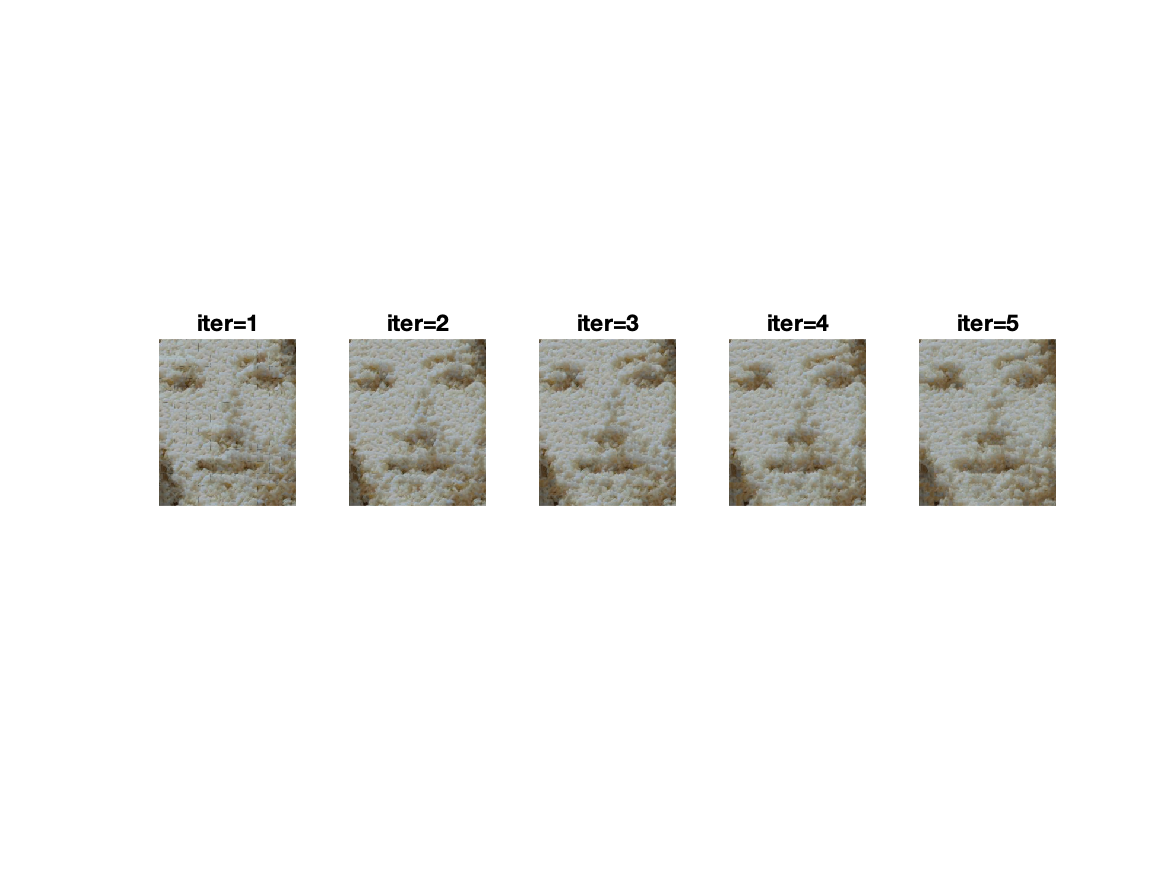
\includegraphics[trim={2cm 6cm 2cm 4cm}, clip, scale=0.9]{../results/iters/res_rice_bill_b_20_bdr_0_800000.png}
    \end{center}
    \vspace{-0.2em}
    \caption{Rice-Bill, iterations, Block size=20, B decay rate = 0.8}
    \label{fig:rice_bill_iter}
\end{figure*}

\begin{figure*}[h]
    \begin{center}
    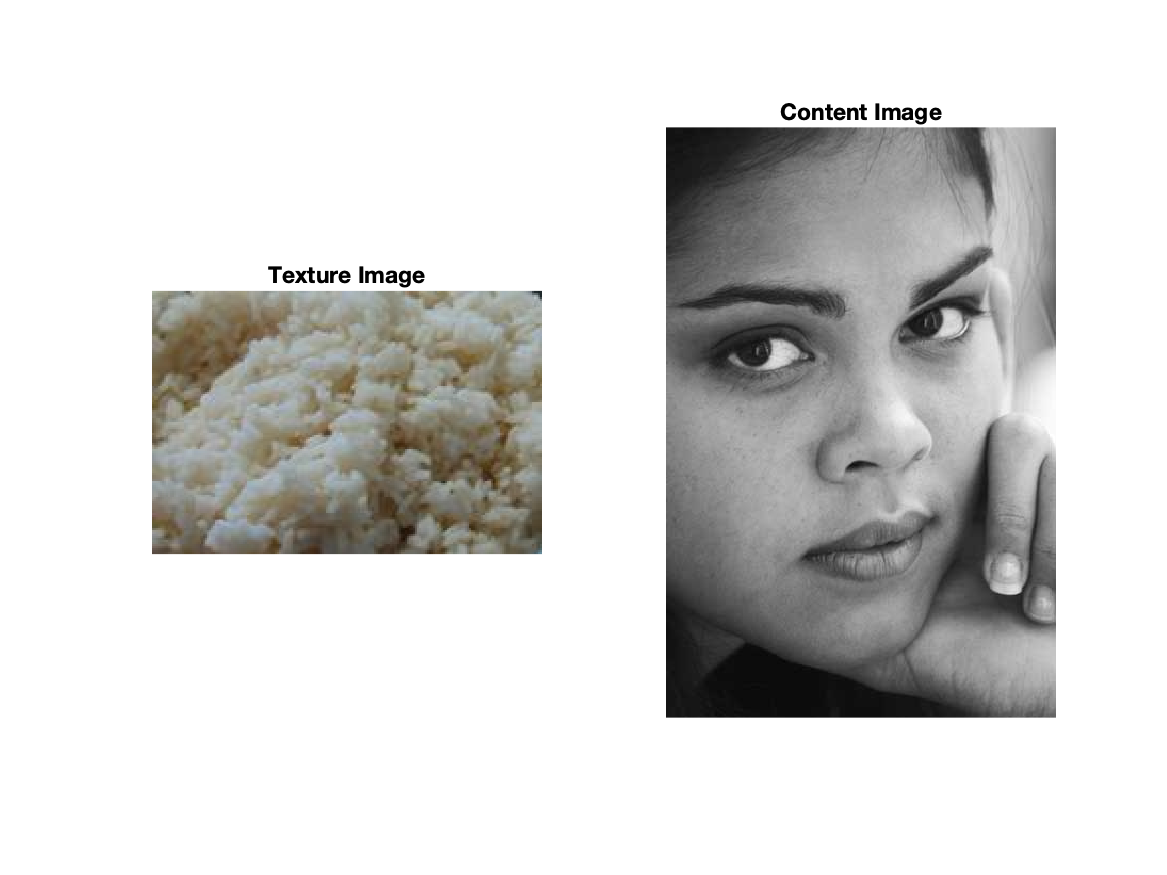
\includegraphics[trim={2cm 4cm 2cm 2cm}, clip, scale=0.5]{../results/bsize/inp_rice_girl.png}
    \end{center}
    \vspace{-0.2em}
    \caption{Rice-Girl}
    \label{fig:rice_girl}
\end{figure*}

\begin{figure*}[h]
    \begin{center}
    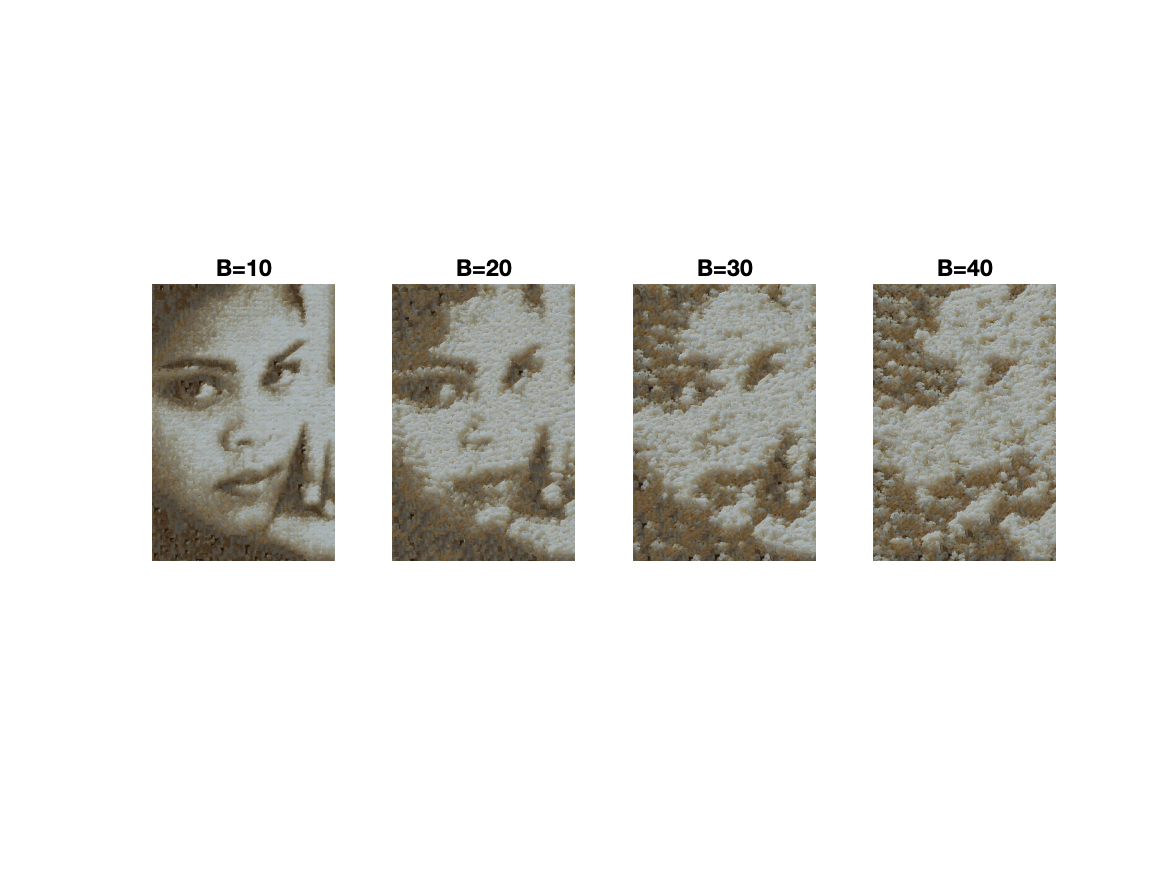
\includegraphics[trim={2cm 6cm 2cm 4cm}, clip, scale=0.9]{../results/bsize/res_rice_girl_bdr_0_700000_iter_5.png}
    \end{center}
    \vspace{-0.2em}
    \caption{Rice-Bill, B decay rate = 0.7}
    \label{fig:rice_girl_bs}
\end{figure*}

% Changes with iteration
\begin{figure*}[h]
    \begin{center}
    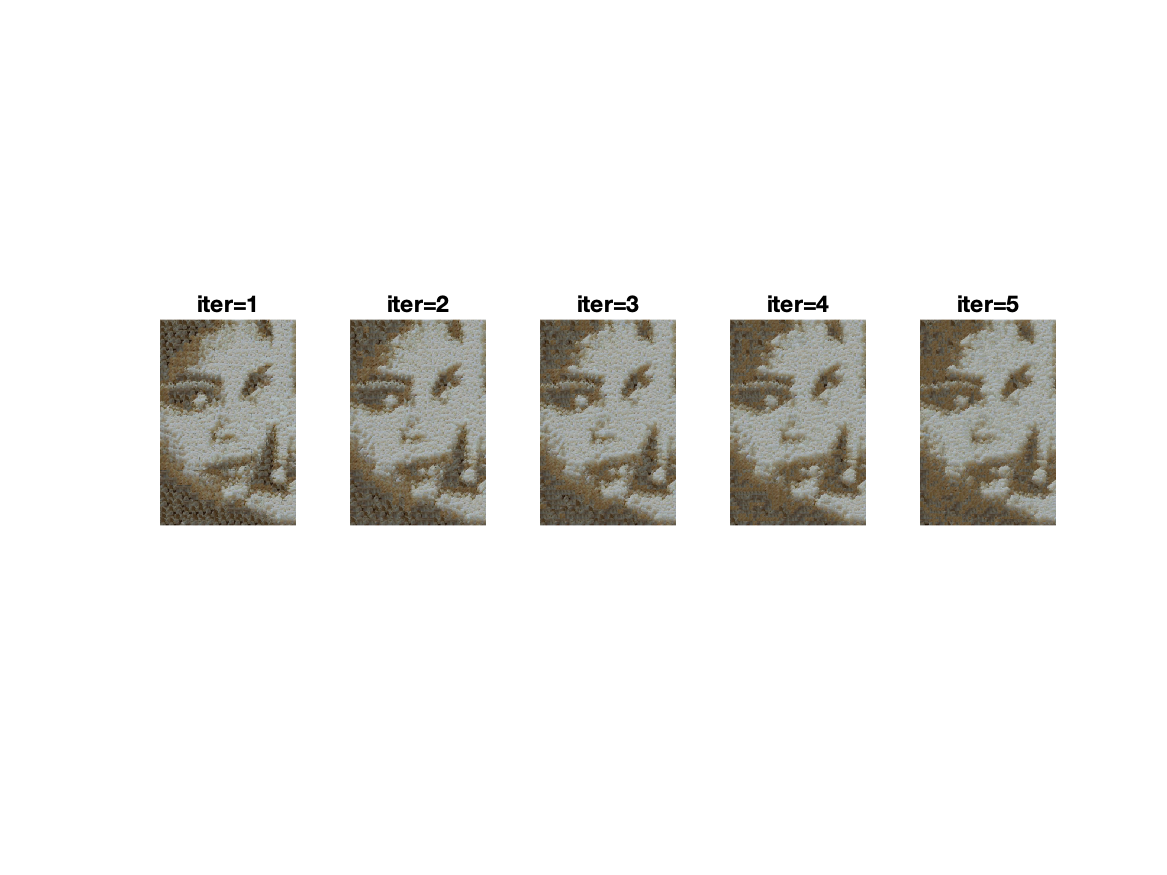
\includegraphics[trim={2cm 6cm 2cm 4cm}, clip, scale=0.9]{../results/iters/res_rice_girl_b_20_bdr_0_800000.png}
    \end{center}
    \vspace{-0.2em}
    \caption{Rice-Girl, iterations, Block size=20, B decay rate = 0.8}
    \label{fig:rice_girl_iter}
\end{figure*}


\begin{figure*}[h]
    \begin{center}
    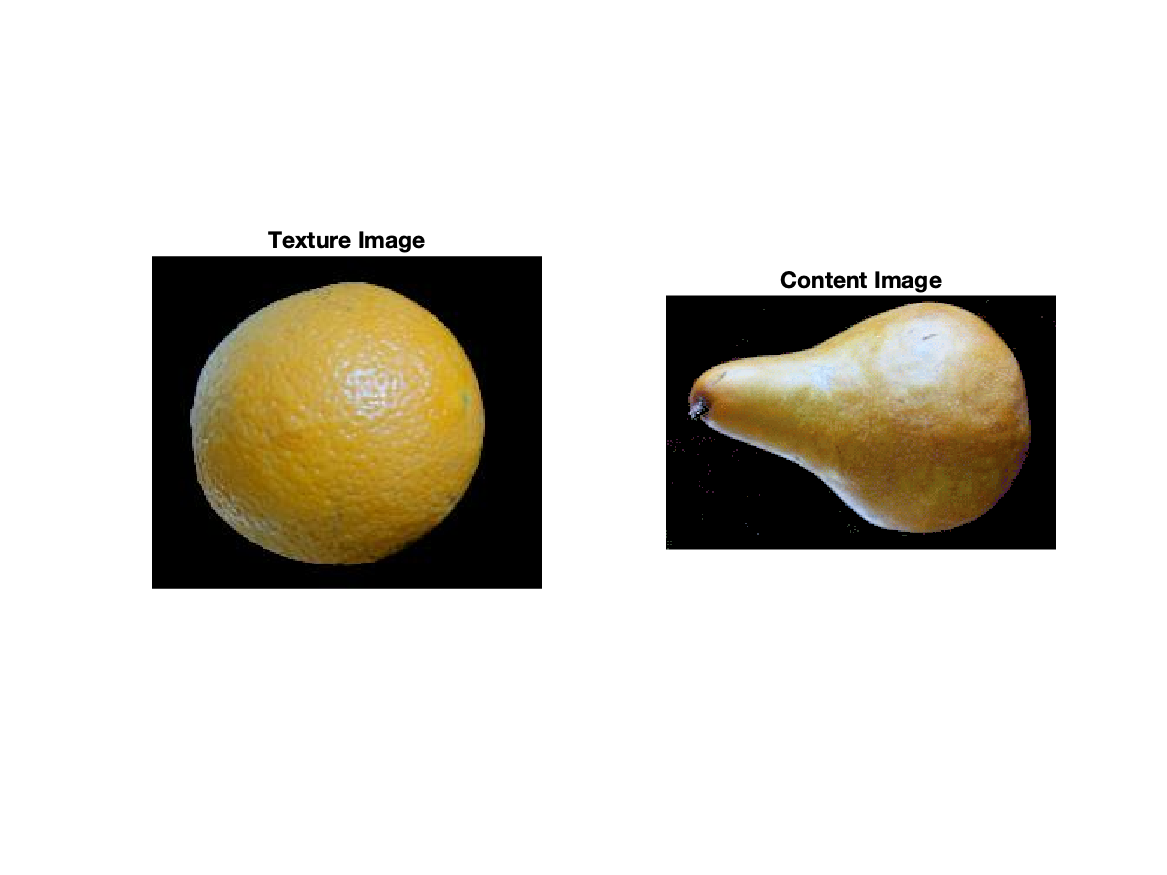
\includegraphics[trim={2cm 4cm 2cm 2cm}, clip, scale=0.5]{../results/bsize/inp_orange_pear.png}
    \end{center}
    \vspace{-0.2em}
    \caption{Orange-Pear}
    \label{fig:or_pear}
\end{figure*}

\begin{figure*}[h]
    \begin{center}
    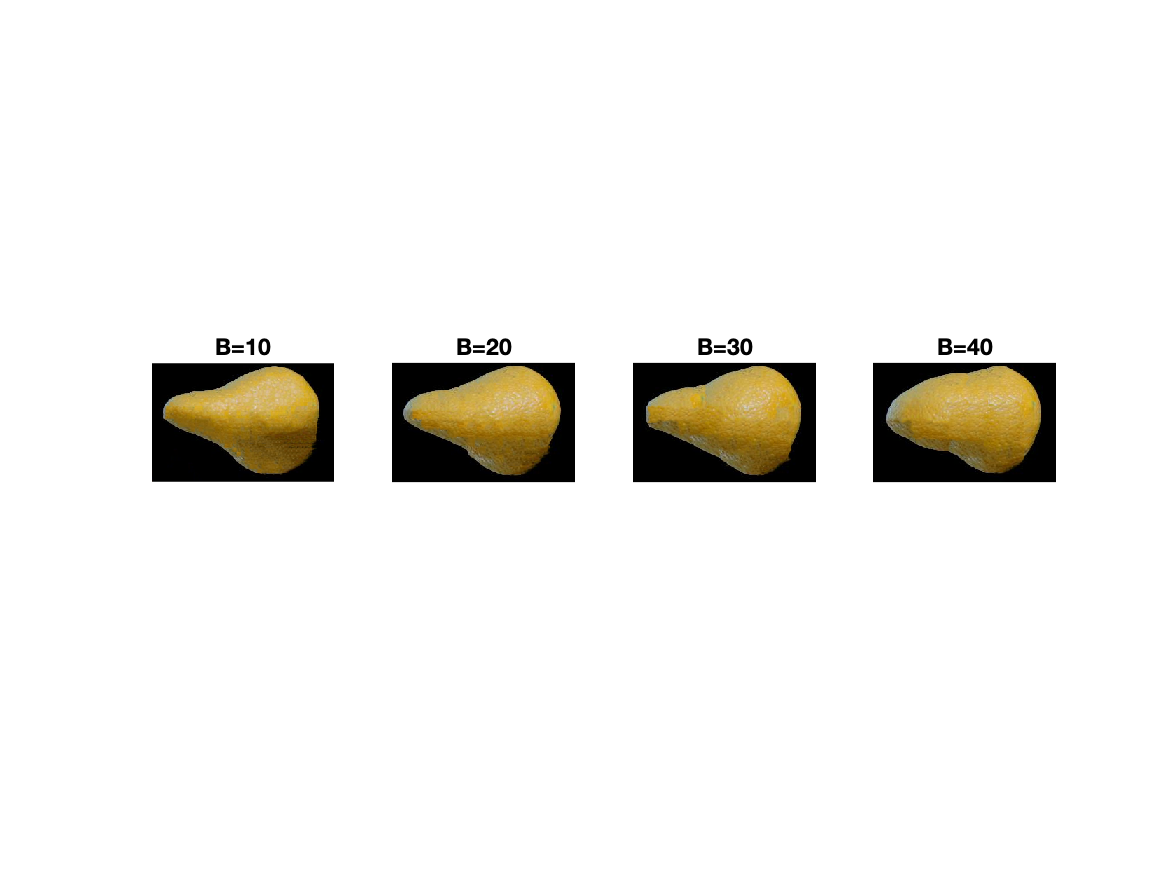
\includegraphics[trim={2cm 6cm 2cm 4cm}, clip, scale=0.9]{../results/bsize/res_orange_pear_bdr_0_900000_iter_5.png}
    \end{center}
    \vspace{-0.2em}
    \caption{Orange-Pear, B decay rate = 0.9}
    \label{fig:orange_pear_bs}
\end{figure*}

% Changes with iteration
\begin{figure*}[h]
    \begin{center}
    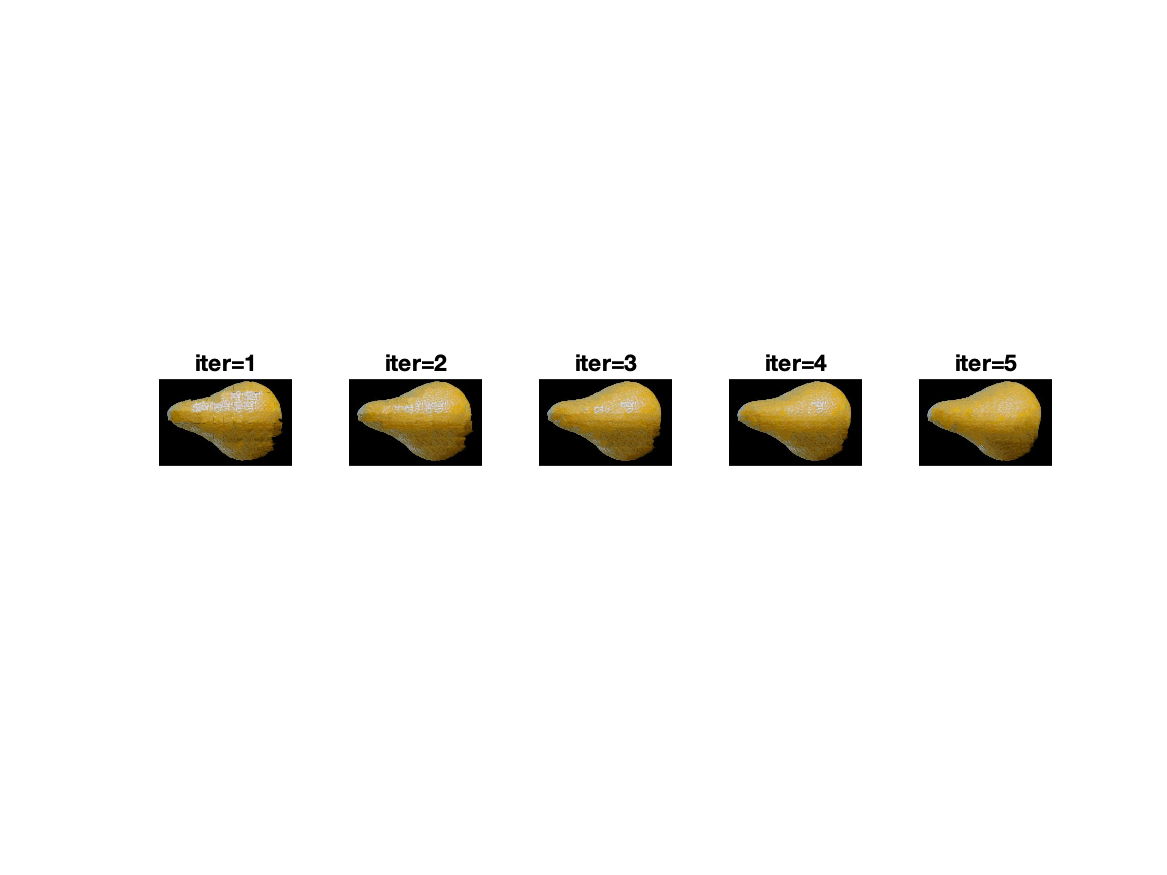
\includegraphics[trim={2cm 6cm 2cm 4cm}, clip, scale=0.9]{../results/iters/res_orange_pear_b_20_bdr_0_800000.png}
    \end{center}
    \vspace{-0.2em}
    \caption{Orange-Pear, iterations, Block size=20, B decay rate = 0.8}
    \label{fig:or_pear_iter}
\end{figure*}


\section{Results \& Conclusion}
We have some amazing synthesis results below followed by transfer results.

\begin{figure*}
     \centering
     \begin{subfigure}[h]{0.33\textwidth}
         \centering
         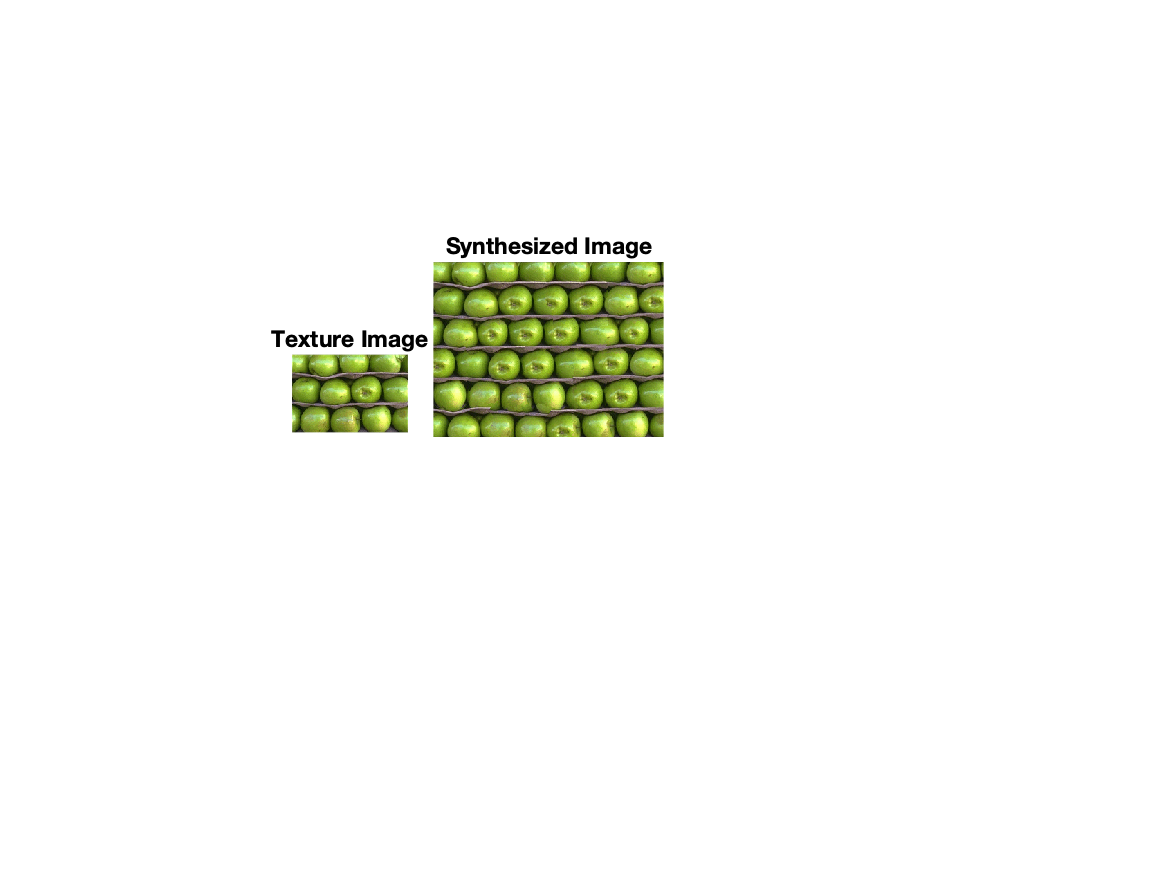
\includegraphics[trim={4.5cm 7cm 8.0cm 3cm}, clip, scale=1.5, width=\textwidth]{../results/syn_final/result_apples_c_B_40.png}
         \caption{Apples}
         \label{fig:apples_res}
     \end{subfigure}
     \hfill
     \begin{subfigure}[h]{0.33\textwidth}
        \centering
        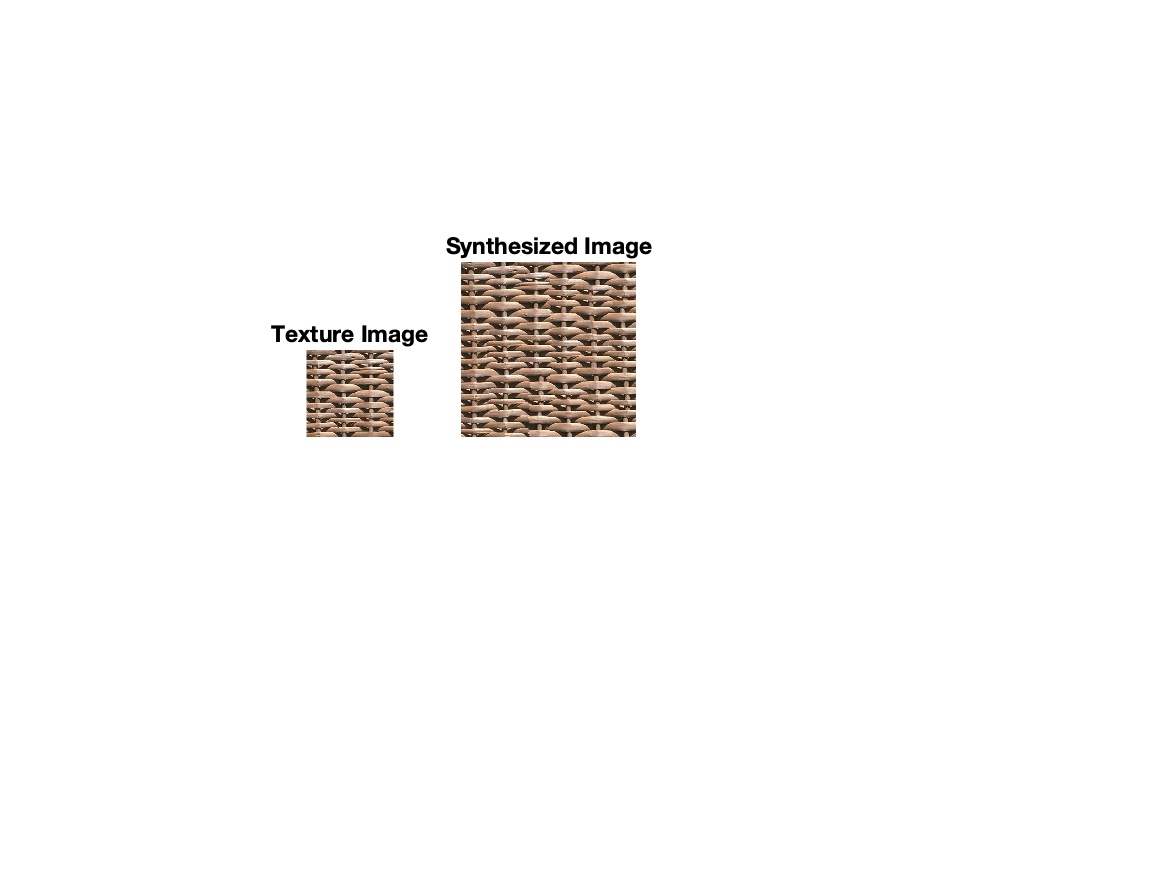
\includegraphics[trim={4.5cm 7cm 8.0cm 3cm}, clip, scale=1.5, width=\textwidth]{../results/syn_final/result_jute_c_B_40.png}
        \caption{Jute}
        \label{fig:jute_res}
    \end{subfigure}
    \hfill
    \begin{subfigure}[h]{0.33\textwidth}
        \centering
        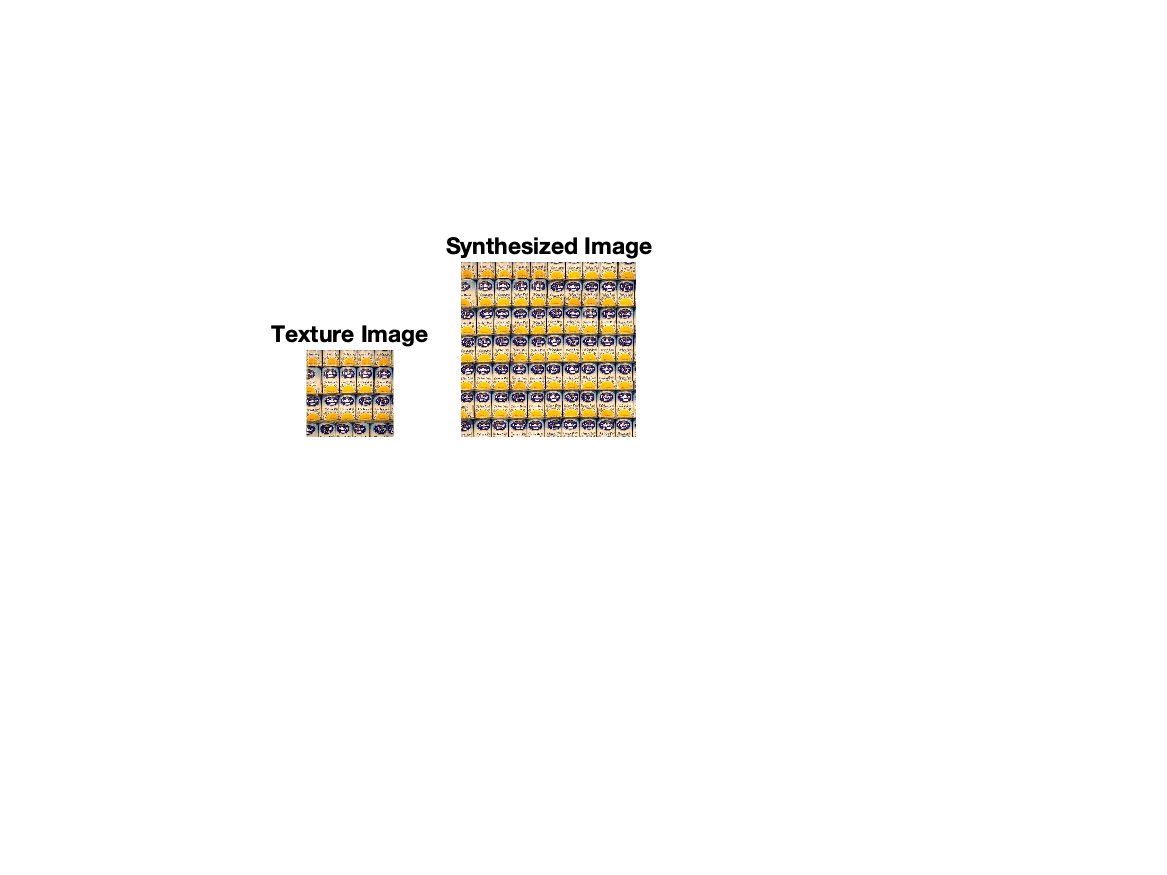
\includegraphics[trim={4.5cm 7cm 8.0cm 3cm}, clip, scale=1.5, width=\textwidth]{../results/syn_final/result_cans_B_80.png}
        \caption{Cans}
        \label{fig:cans_res}
    \end{subfigure}
    \begin{subfigure}[h]{0.33\textwidth}
        \centering
        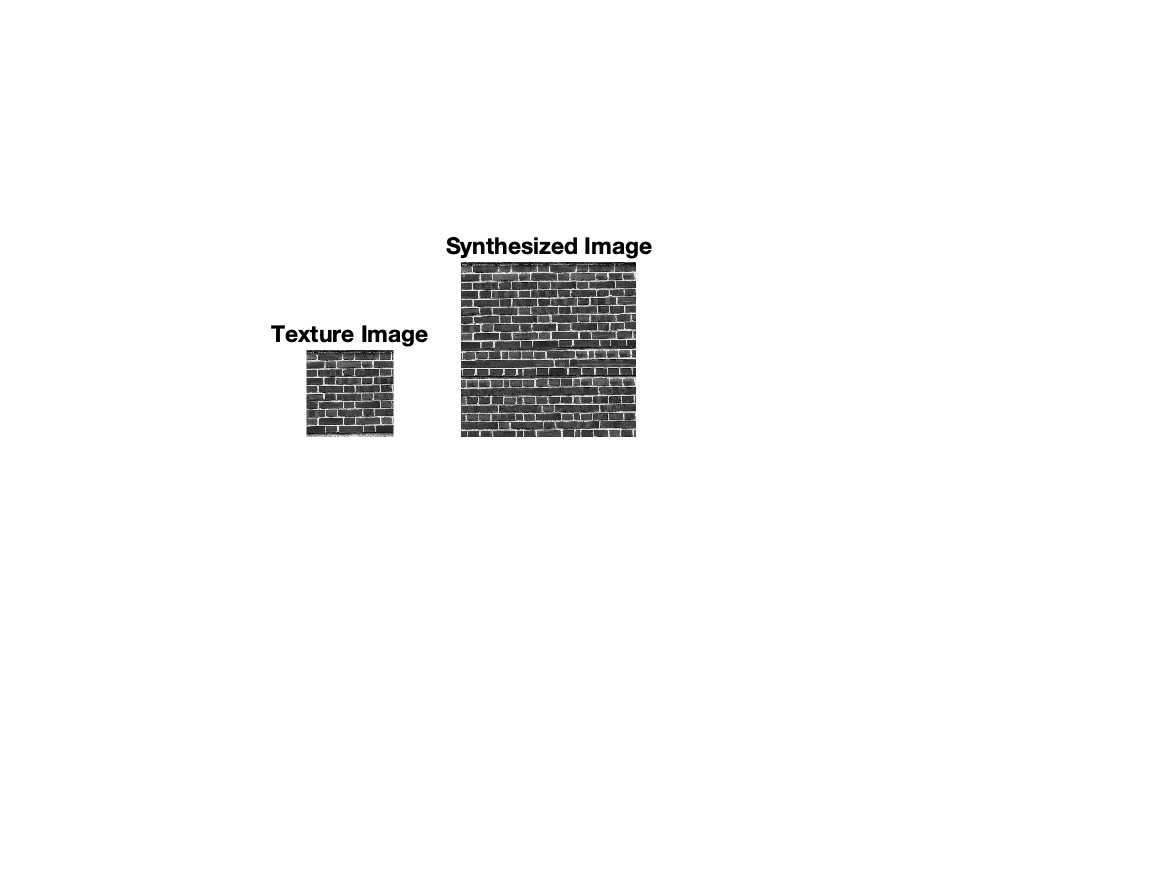
\includegraphics[trim={4.5cm 7cm 8.0cm 3cm}, clip, scale=1.5, width=\textwidth]{../results/syn_final/result_brick_bw_B_40.png}
        \caption{D1}
        \label{fig:d1_res}
    \end{subfigure}
    \hfill
    \begin{subfigure}[h]{0.33\textwidth}
       \centering
       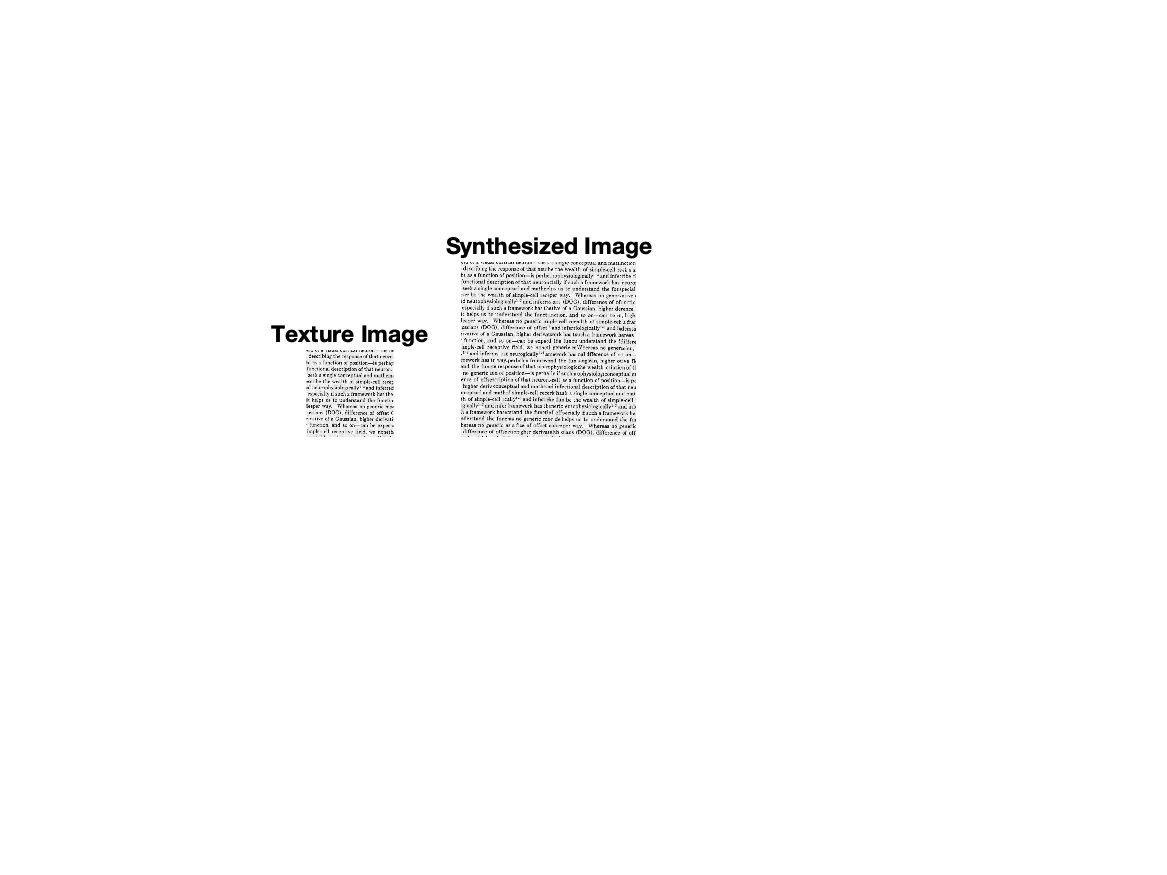
\includegraphics[trim={4.5cm 7cm 8.0cm 3cm}, clip, scale=1.5, width=\textwidth]{../results/syn_final/result_text_B_40.png}
       \caption{text}
       \label{fig:text_res}
   \end{subfigure}
   \hfill
   \begin{subfigure}[h]{0.33\textwidth}
       \centering
       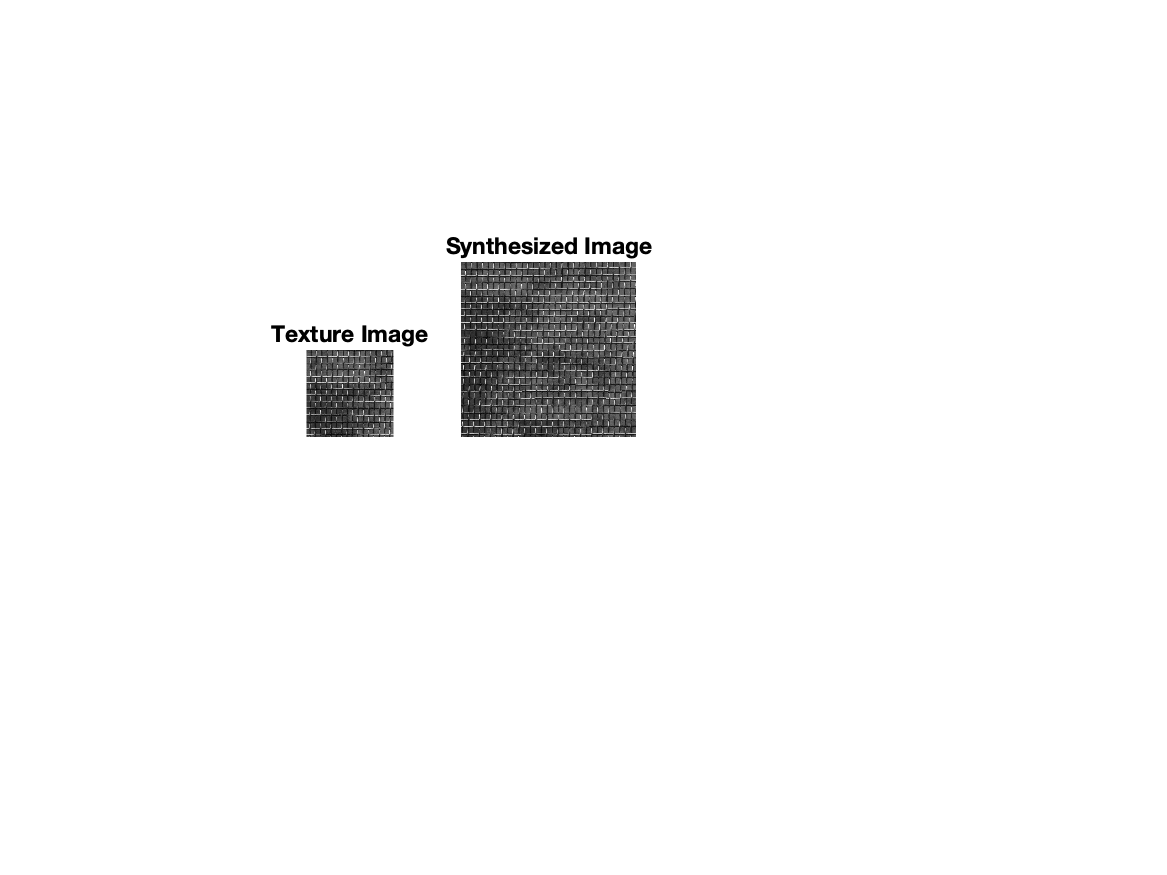
\includegraphics[trim={4.5cm 7cm 8.0cm 3cm}, clip, scale=1.5, width=\textwidth]{../results/syn_final/result_D1_B_40.png}
       \caption{Bricks B/W}
       \label{fig:bricksbw_res}
   \end{subfigure}
   \begin{subfigure}[h]{0.33\textwidth}
         \centering
         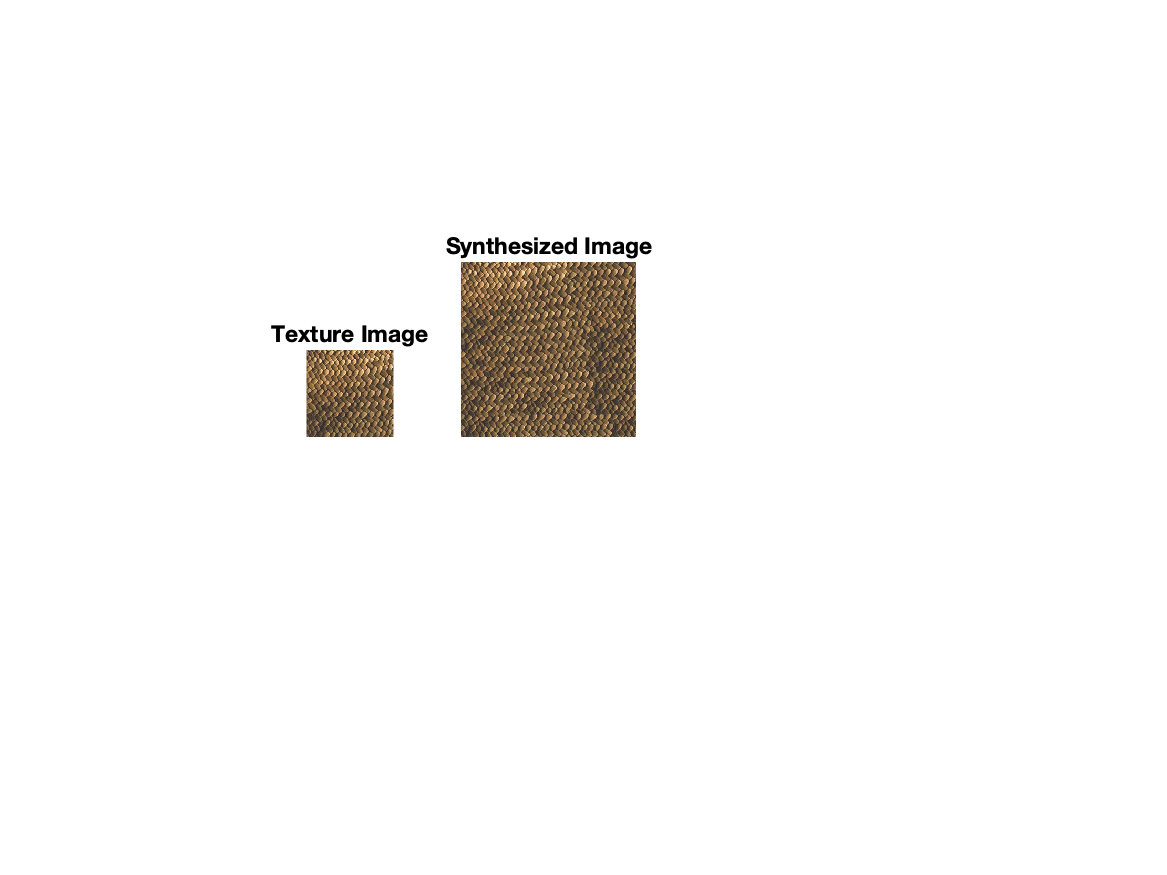
\includegraphics[trim={4.5cm 7cm 8.0cm 3cm}, clip, scale=1.5, width=\textwidth]{../results/syn_final/result_fabric_B_40.png}
         \caption{Fabric}
         \label{fig:apple_res}
     \end{subfigure}
     \hfill
     \begin{subfigure}[h]{0.33\textwidth}
        \centering
        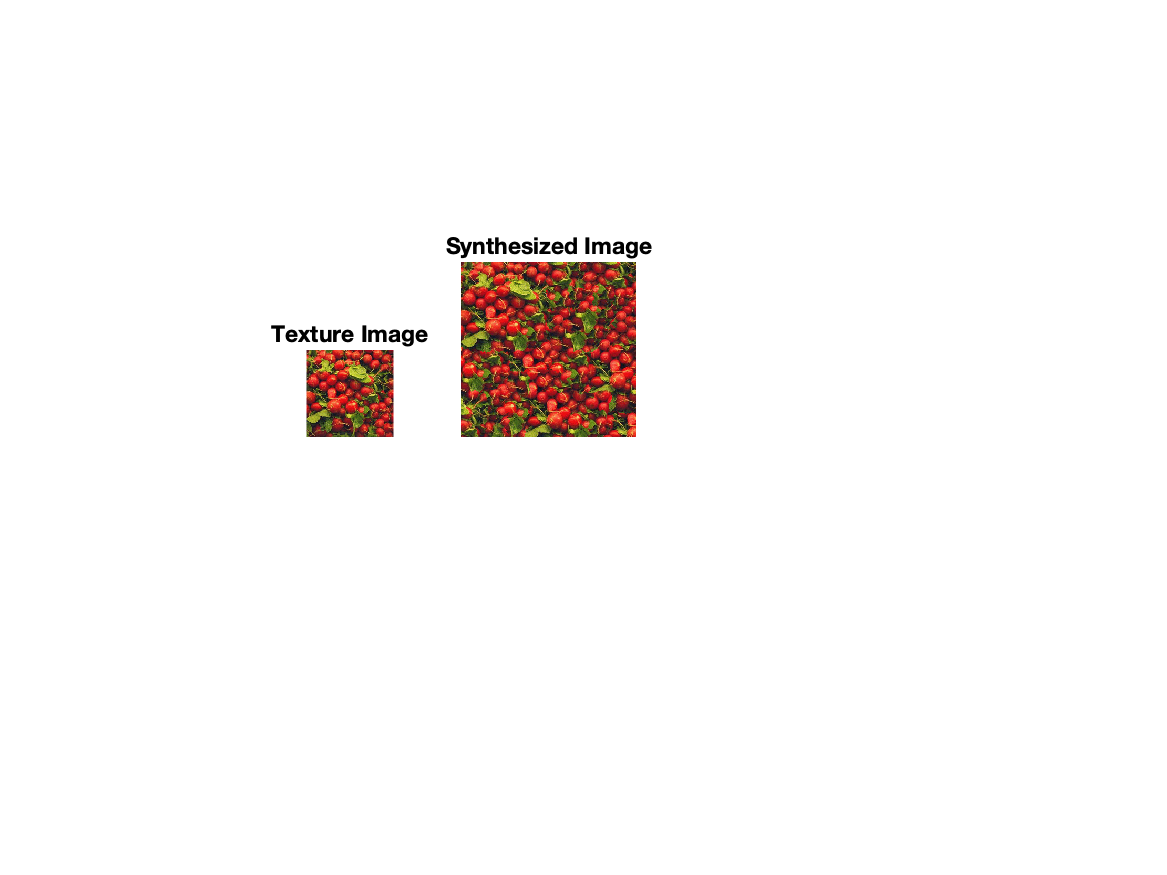
\includegraphics[trim={4.5cm 7cm 8.0cm 3cm}, clip, scale=1.5, width=\textwidth]{../results/syn_final/result_radishes_B_40.png}
        \caption{Radishes}
        \label{fig:apple_res}
    \end{subfigure}
    \hfill
    \begin{subfigure}[h]{0.33\textwidth}
        \centering
        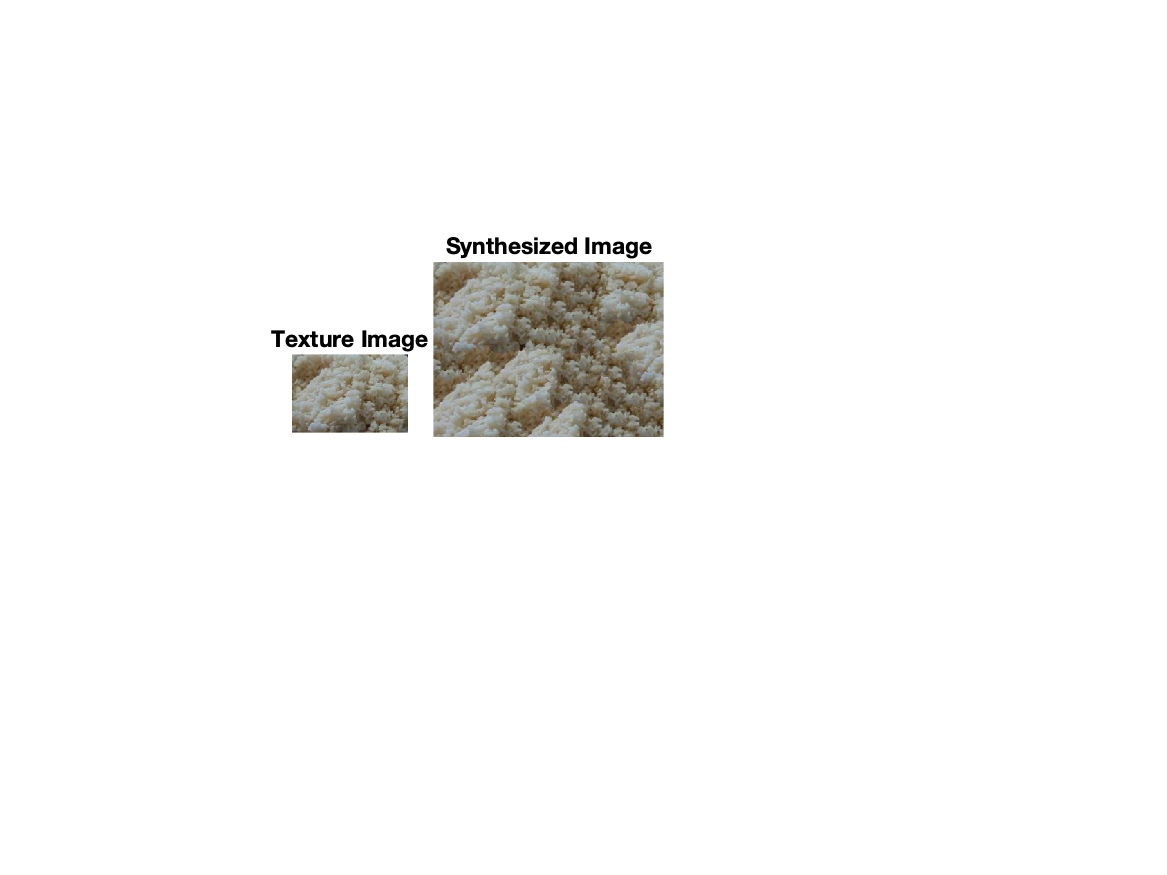
\includegraphics[trim={4.5cm 7cm 8.0cm 3cm}, clip, scale=1.5, width=\textwidth]{../results/syn_final/result_rice_B_40.png}
        \caption{Rice}
        \label{fig:apple_res}
    \end{subfigure}
    \begin{subfigure}[h]{0.33\textwidth}
        \centering
        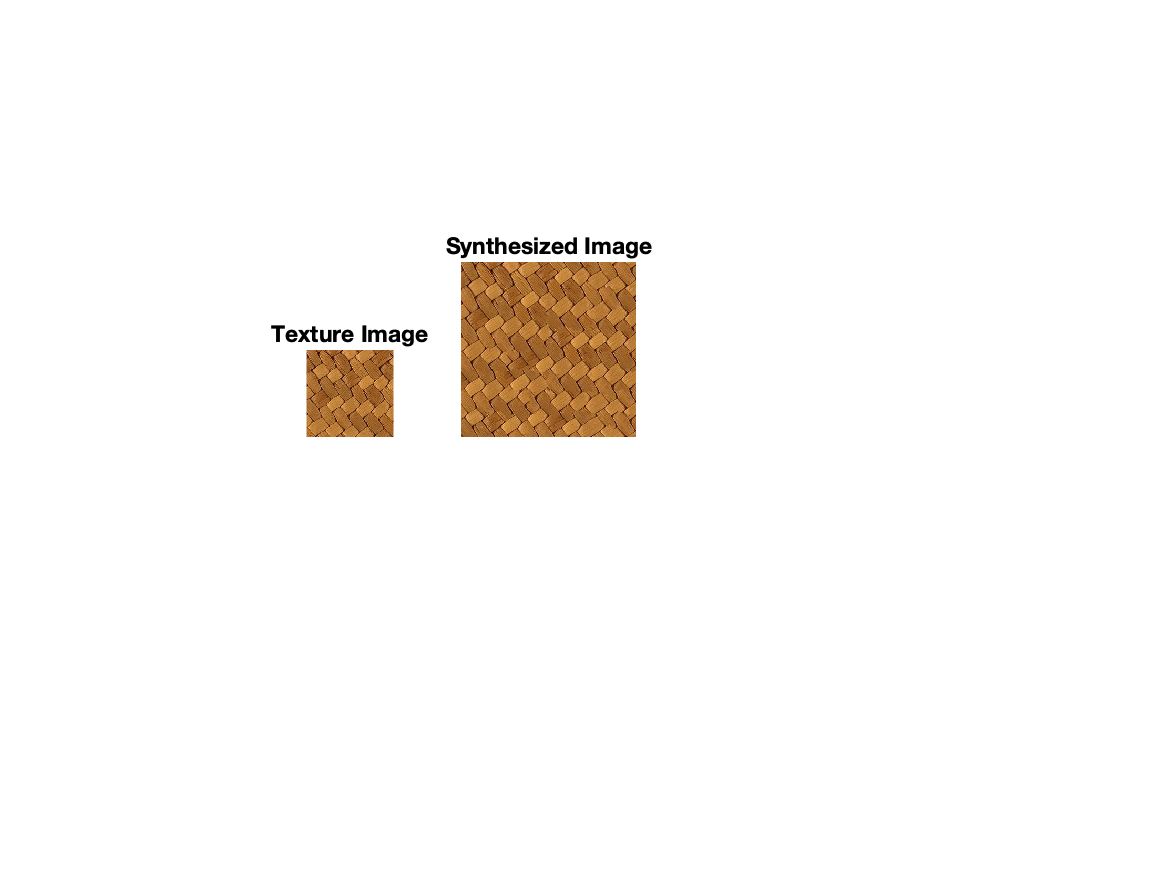
\includegraphics[trim={4.5cm 7cm 8.0cm 3cm}, clip, scale=1.5, width=\textwidth]{../results/syn_final/result_wood_c_B_40.png}
        \caption{Wood}
        \label{fig:apple_res}
    \end{subfigure}
    \hfill
    \begin{subfigure}[h]{0.33\textwidth}
       \centering
       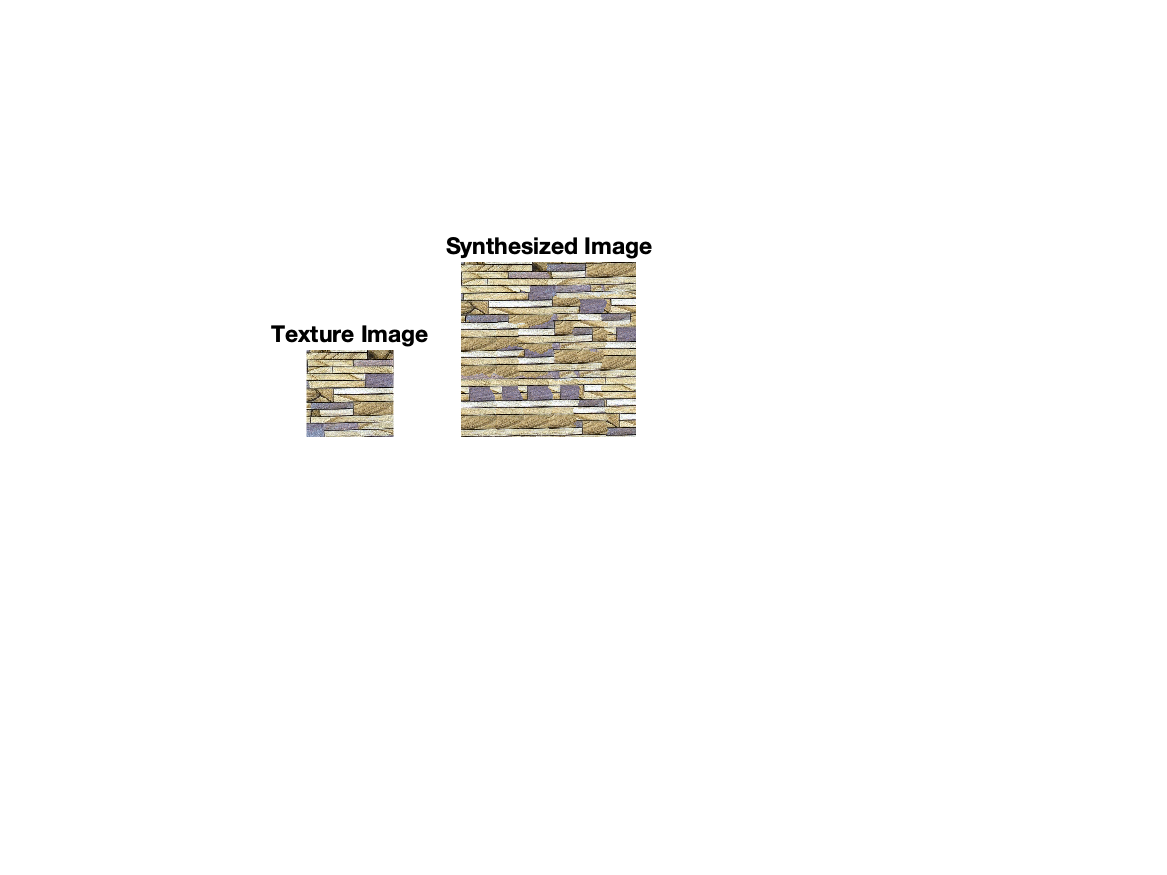
\includegraphics[trim={4.5cm 7cm 8.0cm 3cm}, clip, scale=1.5, width=\textwidth]{../results/syn_final/result_tile_B_60.png}
       \caption{Tiles}
       \label{fig:apple_res}
   \end{subfigure}
   \hfill
   \begin{subfigure}[h]{0.33\textwidth}
       \centering
       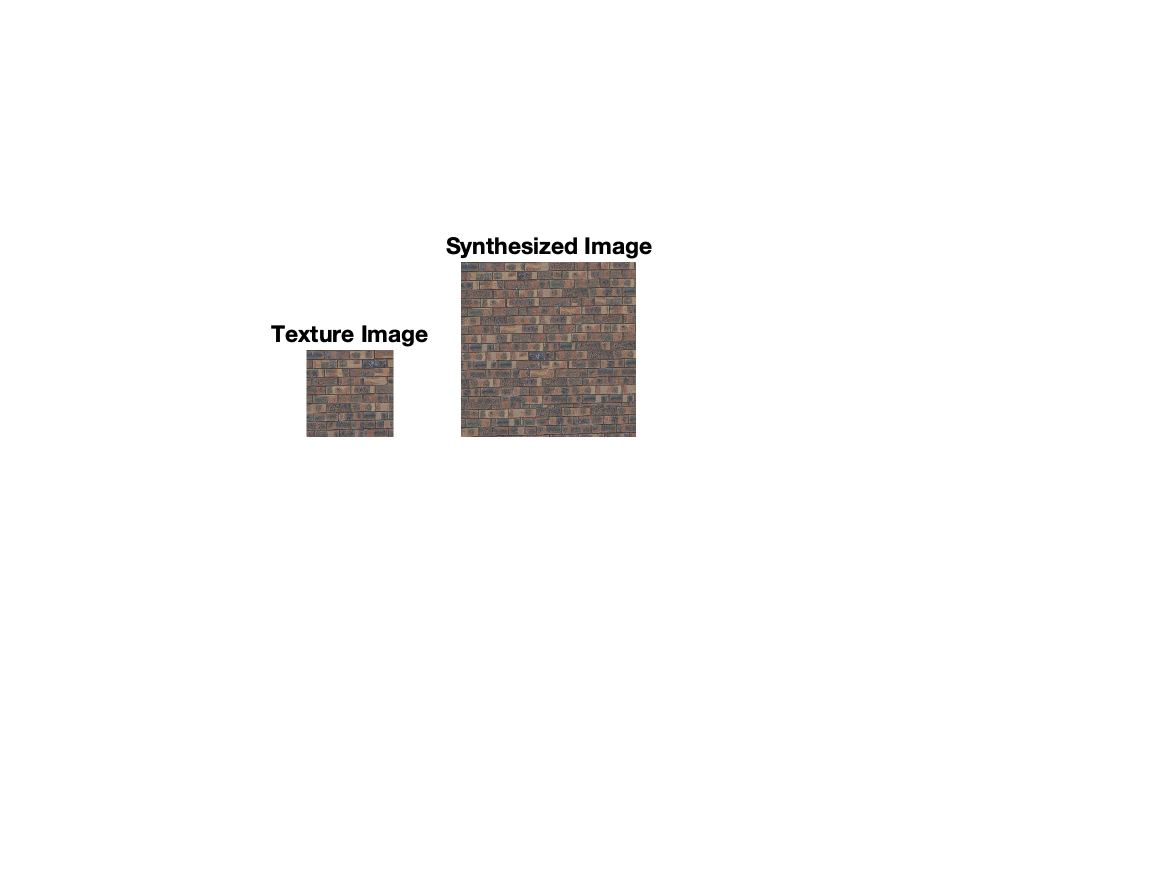
\includegraphics[trim={4.5cm 7cm 8.0cm 3cm}, clip, scale=1.5, width=\textwidth]{../results/syn_final/result_brick_B_60.png}
       \caption{Bricks}
       \label{fig:apple_res}
   \end{subfigure}
   \begin{subfigure}[h]{0.33\textwidth}
    \centering
    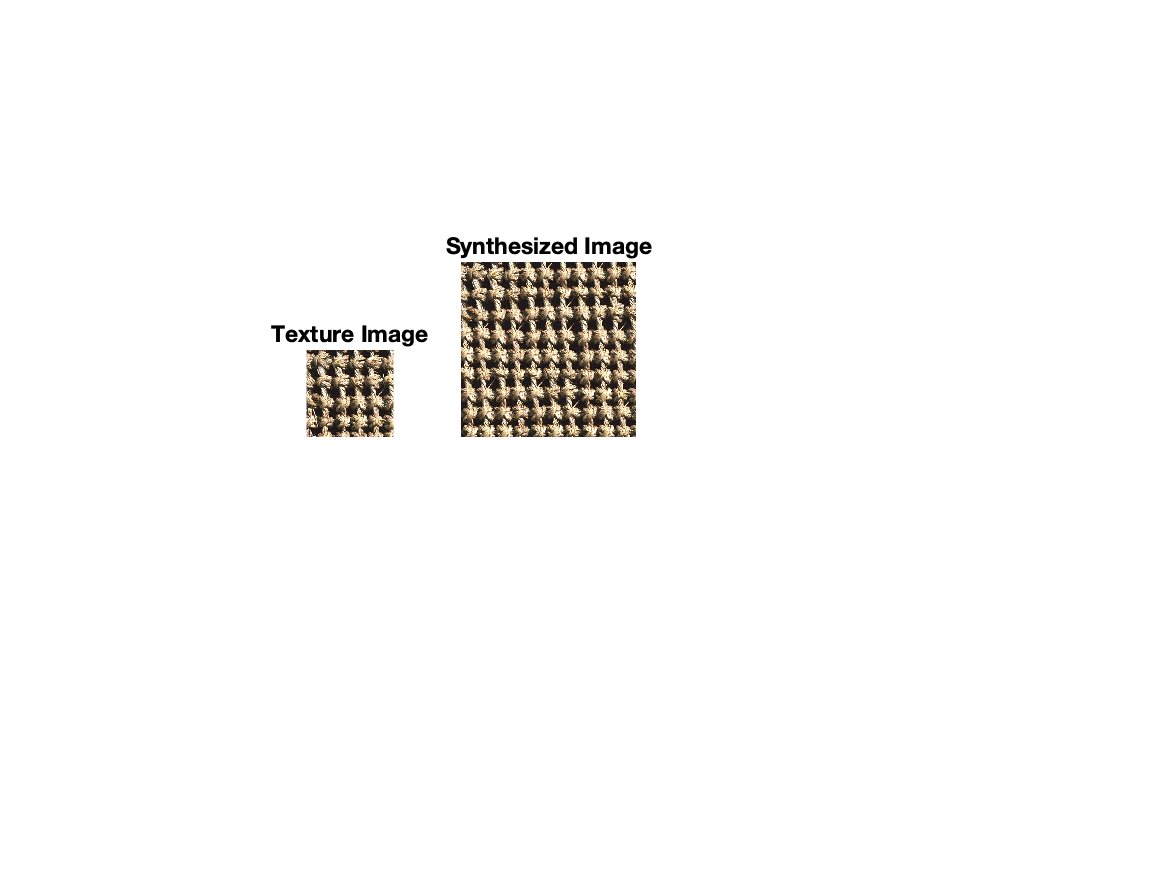
\includegraphics[trim={4.5cm 7cm 8.0cm 3cm}, clip, scale=1.5, width=\textwidth]{../results/syn_final/result_rope_B_60.png}
    \caption{Rope}
    \label{fig:apple_res}
\end{subfigure}
\hfill
\begin{subfigure}[h]{0.33\textwidth}
   \centering
   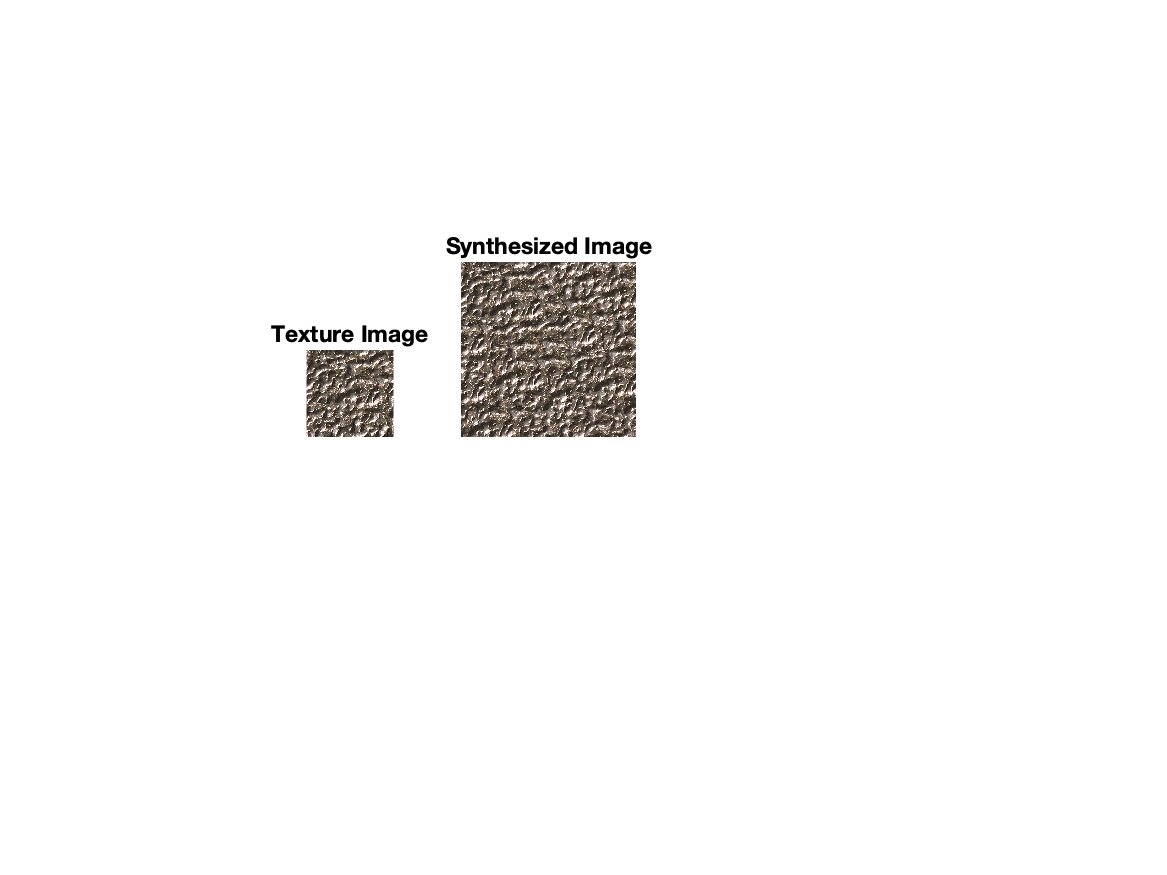
\includegraphics[trim={4.5cm 7cm 8.0cm 3cm}, clip, scale=1.5, width=\textwidth]{../results/syn_final/result_br_pattern_B_60.png}
   \caption{Pattern}
   \label{fig:apple_res}
\end{subfigure}
\hfill
\begin{subfigure}[h]{0.33\textwidth}
   \centering
   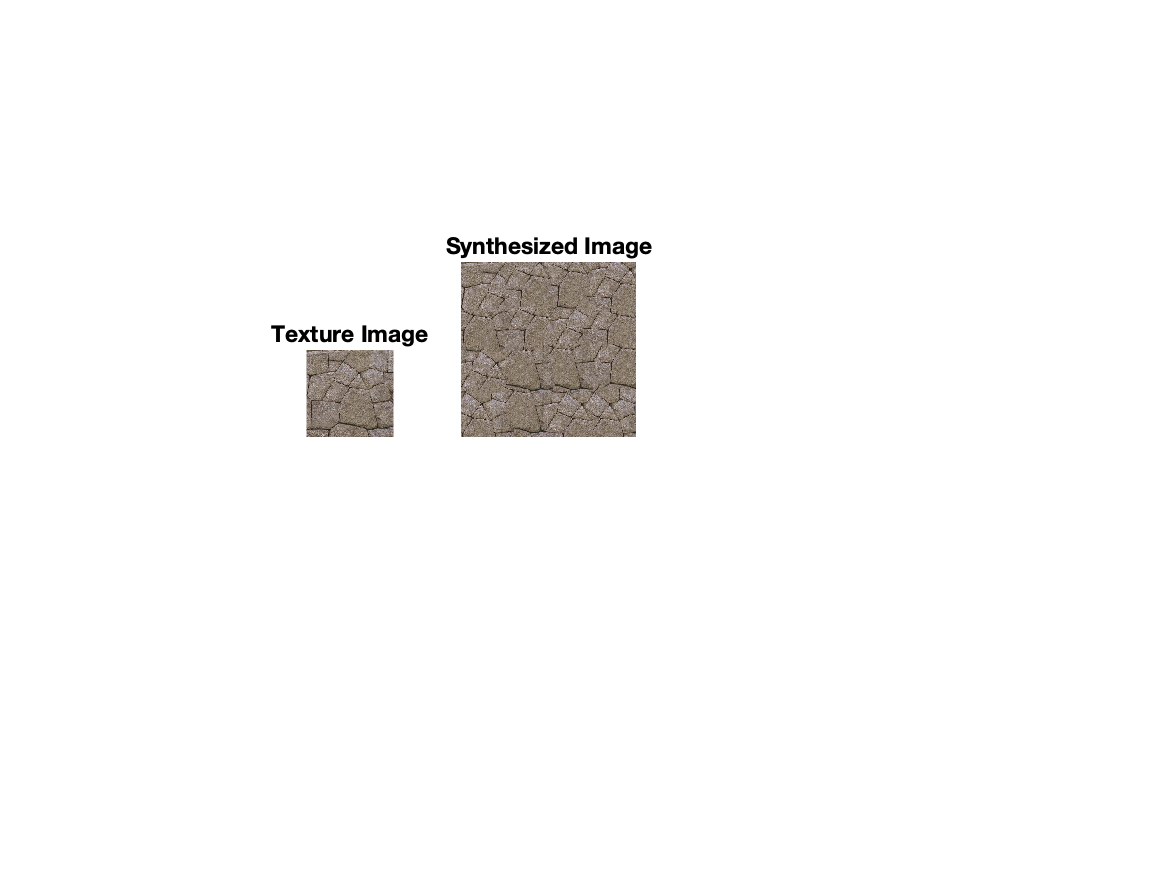
\includegraphics[trim={4.5cm 7cm 8.0cm 3cm}, clip, scale=1.5, width=\textwidth]{../results/syn_final/result_stone_B_90.png}
   \caption{Stone}
   \label{fig:apple_res}
\end{subfigure}   
       \caption{Quilting Results}
        \label{fig:quil_final}
\end{figure*}


\begin{figure*}[h]
    \centering
    \begin{subfigure}[h]{0.4\textwidth}
        \centering
        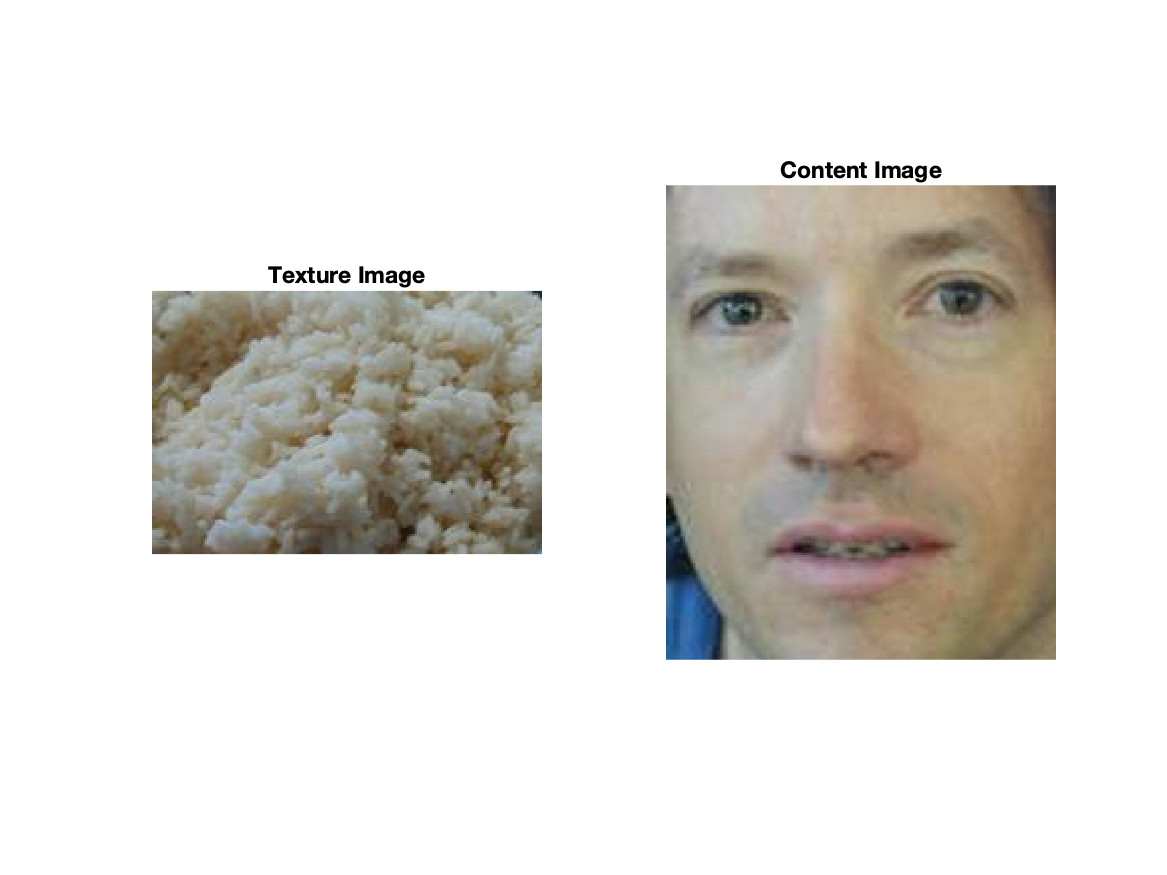
\includegraphics[trim={2cm 4cm 2cm 2cm}, clip, scale=0.5]{../results/bsize/inp_rice_bill.png}
        \caption{Input}
    \end{subfigure}
    \hfill
    \begin{subfigure}[h]{0.5\textwidth}
       \centering
       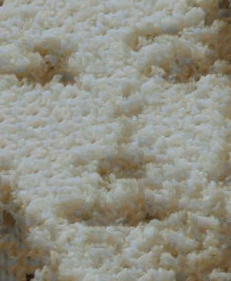
\includegraphics[scale=0.6]{../results/bsize/out_rice_bill_B_20_bdr_0_800000.png}
       \caption{Output}
   \end{subfigure}
   \caption{Result for Rice-Bill}
   \label{fig:ap_bs}
\end{figure*}

\begin{figure*}[h]
    \centering
    \begin{subfigure}[h]{0.45\textwidth}
        \centering
        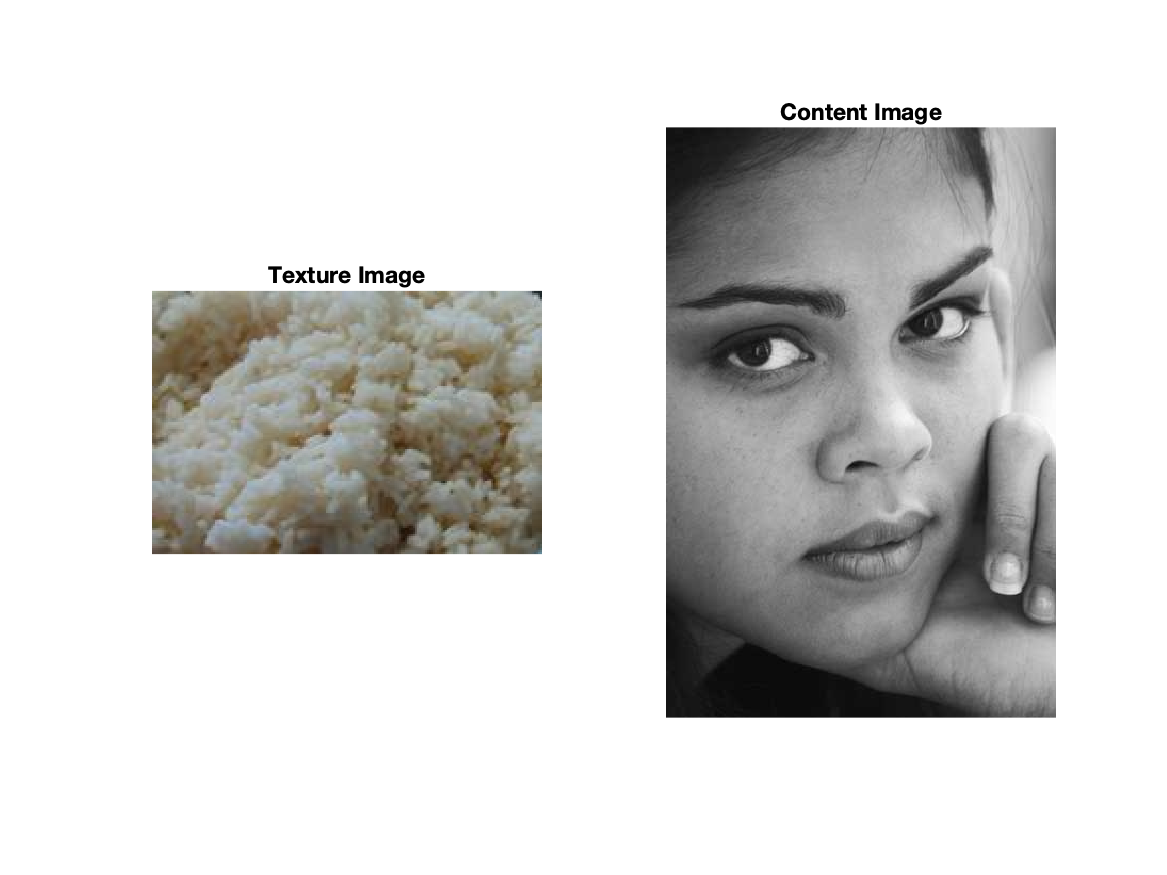
\includegraphics[trim={2cm 4cm 2cm 1cm}, clip, scale=0.5]{../results/bsize/inp_rice_girl.png}
        \caption{Input}
    \end{subfigure}
    \hfill
    \begin{subfigure}[h]{0.5\textwidth}
       \centering
       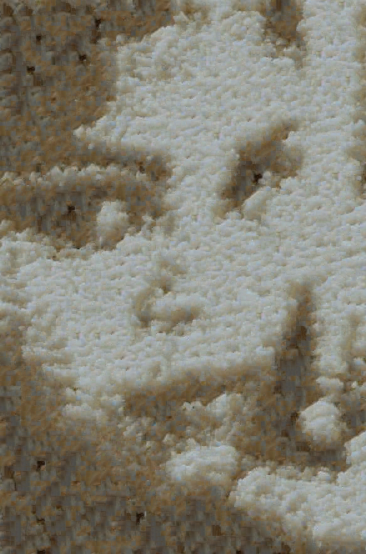
\includegraphics[scale=0.4]{../results/bsize/out_rice_girl_B_20_bdr_0_700000.png}
       \caption{Output}
   \end{subfigure}
   \caption{Result for Rice-Girl}
   \label{fig:ap_bs}
\end{figure*}

\begin{figure*}[h]
    \centering
    \begin{subfigure}[h]{0.45\textwidth}
        \centering
        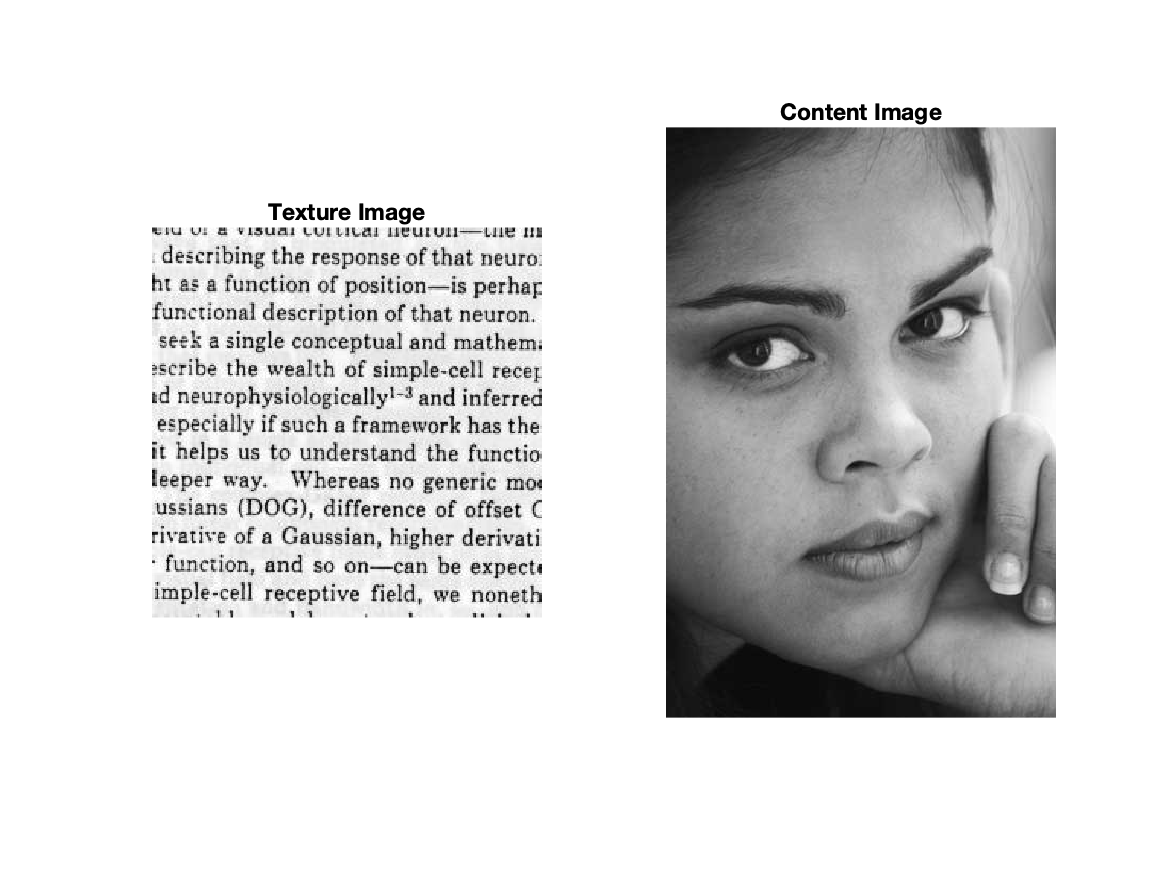
\includegraphics[trim={2cm 4cm 2cm 1cm}, clip, scale=0.5]{../results/bsize/inp_text_girl.png}
        \caption{Input}
    \end{subfigure}
    \hfill
    \begin{subfigure}[h]{0.5\textwidth}
       \centering
       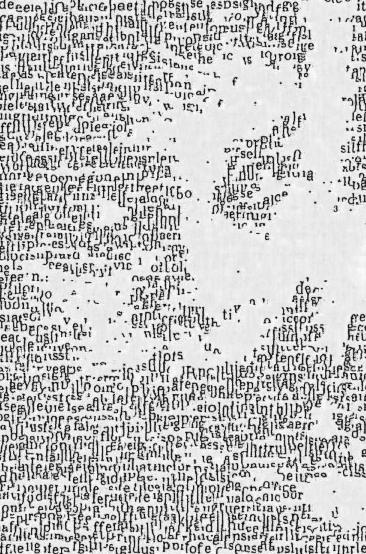
\includegraphics[scale=0.4]{../results/bsize/out_text_girl_B_10_bdr_0_700000.png}`'
       \caption{Output}
   \end{subfigure}
   \caption{Result for Text-Girl}
   \label{fig:ap_bs}
\end{figure*}

\begin{figure*}[h]
    \centering
    \begin{subfigure}[h]{0.45\textwidth}
        \centering
        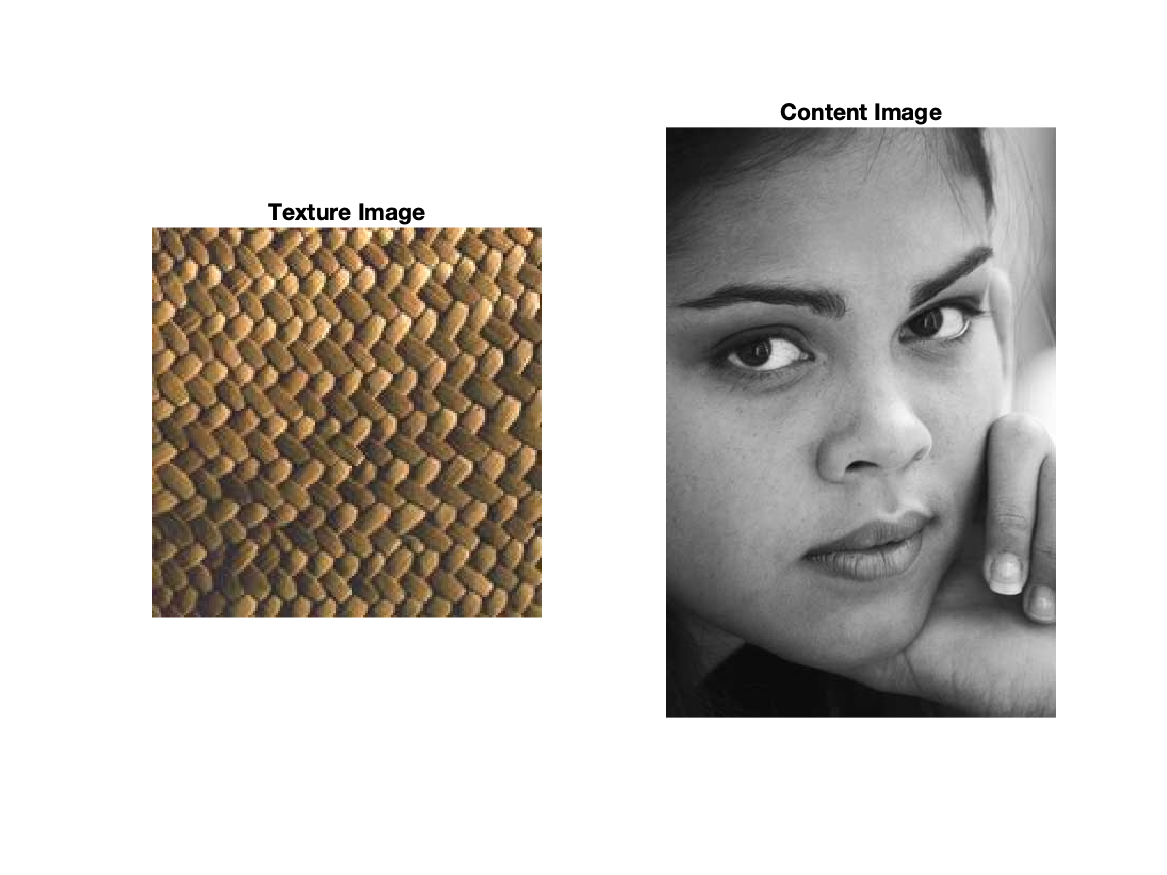
\includegraphics[trim={2cm 4cm 2cm 1cm}, clip, scale=0.5]{../results/bsize/inp_fabric_girl.png}
        \caption{Input}
    \end{subfigure}
    \hfill
    \begin{subfigure}[h]{0.5\textwidth}
       \centering
       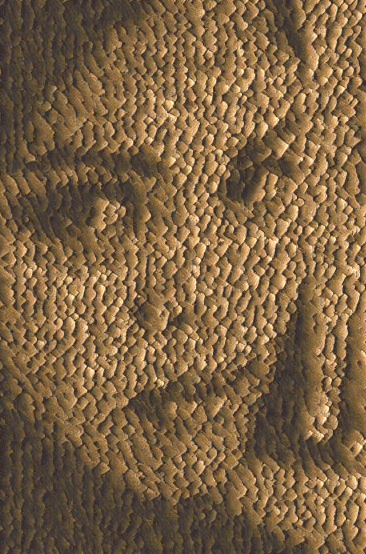
\includegraphics[scale=0.4]{../results/bsize/out_fabric_girl_B_10_bdr_0_800000.png}
       \caption{Output}
   \end{subfigure}
   \caption{Result for Fabric-Girl}
   \label{fig:ap_bs}
\end{figure*}

\begin{figure*}[h]
    \centering
    \begin{subfigure}[h]{0.45\textwidth}
        \centering
        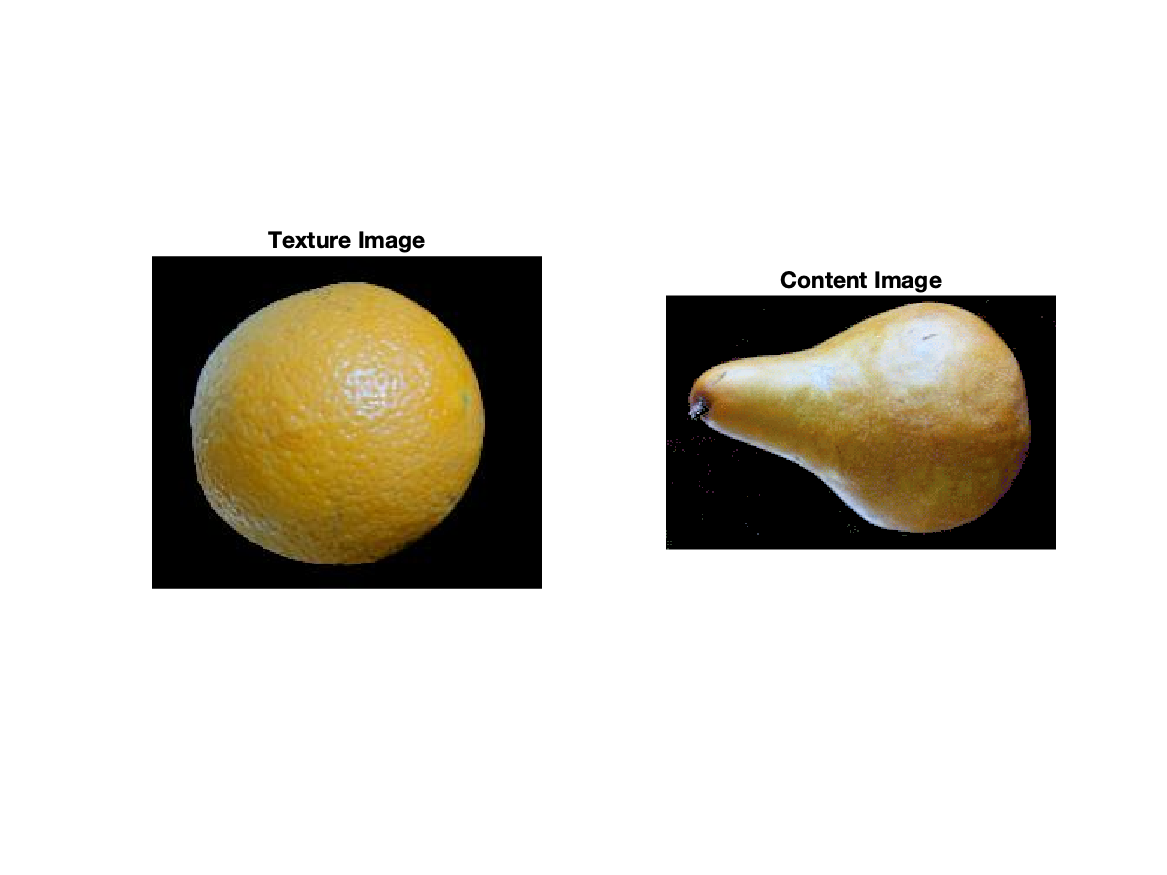
\includegraphics[trim={2cm 4cm 2cm 3cm}, clip, scale=0.5]{../results/bsize/inp_orange_pear.png}
        \caption{Input}
    \end{subfigure}
    \hfill
    \begin{subfigure}[h]{0.5\textwidth}
       \centering
       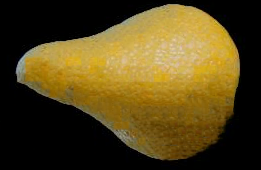
\includegraphics[scale=0.4]{../results/bsize/out_orange_pear_B_20_bdr_0_800000.png}
       \caption{Output}
   \end{subfigure}
   \caption{Result for Orange-Pear}
   \label{fig:ap_bs}
\end{figure*}

\begin{figure*}[h]
    \centering
    \begin{subfigure}[h]{0.45\textwidth}
        \centering
        \includegraphics[trim={2cm 4cm 2cm 3cm}, clip, scale=0.5]{../results/bsize/inp_orange_potato.png}
        \caption{Input}
    \end{subfigure}
    \hfill
    \begin{subfigure}[h]{0.5\textwidth}
       \centering
       \includegraphics[scale=0.4]{../results/bsize/out_orange_potato_B_10_bdr_0_700000.png}
       \caption{Output}
   \end{subfigure}
   \caption{Result for Orange-Potato}
   \label{fig:ap_bs}
\end{figure*}

% \begin{thebibliography}{999}

% \bibitem{one}
% https://www.geeksforgeeks.org/deep-q-learning/

% \bibitem{two}
% https://www.cs.swarthmore.edu/~bryce/cs63/s16/slides/3-25approximateQ-learning.pdf
% main ref for QL: 
% \bibitem{three}
% http://www.gatsby.ucl.ac.uk/~dayan/papers/cjch.pdf
% \bibitem{four}
% https://courses.cs.washington.edu/courses/cse473/16au/slides-16au/18-approx-rl2.pdf
% \bibitem{five}
% https://www.intel.ai/demystifying-deep-reinforcement-learning/\#gs.hxyudi
% \bibitem{six}
% https://pdfs.semanticscholar.org/2d7e/7d809af7d68c.pdf
% \bibitem{seven}
% https://github.com/moduIo/Deep-Q-network
% \bibitem{eight}
% https://towardsdatascience.com/advanced-dqns-playing-pac-man-with-deep-reinforcement-learning-3ffbd99e0814
% \bibitem{nine}
% {https://lilianweng.github.io/lil-log/2018/05/05/implementing-deep-reinforcement-learning-models.html}
% \bibitem{ten}{https://gym.openai.com/envs/MsPacman-v0/}
% \bibitem{eleven}{https://github.com/gauravmittal1995/Pyman}
% \bibitem{twelve}{https://pythonprogramming.net/pygame-python-3-part-1-intro/}
% \bibitem{thirteen}{https://oregonstate.instructure.com }
% \end{thebibliography}
\end{document}
